\documentclass[polish, 10pt]{article}
\usepackage{polski}
%%%%%%%%%%%%%%%%%%%%%%%%%%%%%%%%%%%%%%%%%
% Lachaise Assignment
% Structure Specification File
% Version 1.0 (26/6/2018)
%
% This template originates from:
% http://www.LaTeXTemplates.com
%
% Authors:
% Marion Lachaise & François Févotte
% Vel (vel@LaTeXTemplates.com)
%
% License:
% CC BY-NC-SA 3.0 (http://creativecommons.org/licenses/by-nc-sa/3.0/)
%
%%%%%%%%%%%%%%%%%%%%%%%%%%%%%%%%%%%%%%%%%

%----------------------------------------------------------------------------------------
%	PACKAGES AND OTHER DOCUMENT CONFIGURATIONS
%----------------------------------------------------------------------------------------

\usepackage{amsmath,amsfonts,stmaryrd,amssymb} % Math packages

\usepackage{xcolor}
\usepackage{listings}

\usepackage{xparse}

\usepackage{enumerate} % Custom item numbers for enumerations

\usepackage[ruled]{algorithm2e} % Algorithms

\usepackage[framemethod=tikz]{mdframed} % Allows defining custom boxed/framed environments

\usepackage{listings} % File listings, with syntax highlighting
\lstset{
	basicstyle=\ttfamily, % Typeset listings in monospace font
}

%----------------------------------------------------------------------------------------
%	DOCUMENT MARGINS
%----------------------------------------------------------------------------------------

\usepackage{geometry} % Required for adjusting page dimensions and margins

\geometry{
	paper=a4paper, % Paper size, change to letterpaper for US letter size
	top=2.5cm, % Top margin
	bottom=3cm, % Bottom margin
	left=2.5cm, % Left margin
	right=2.5cm, % Right margin
	headheight=14pt, % Header height
	footskip=1.5cm, % Space from the bottom margin to the baseline of the footer
	headsep=1.2cm, % Space from the top margin to the baseline of the header
	%showframe, % Uncomment to show how the type block is set on the page
}

%----------------------------------------------------------------------------------------
%	FONTS
%----------------------------------------------------------------------------------------

\usepackage[utf8]{inputenc} % Required for inputting international characters
\usepackage[T1]{fontenc} % Output font encoding for international characters

\usepackage{XCharter} % Use the XCharter fonts

%----------------------------------------------------------------------------------------
%	COMMAND LINE ENVIRONMENT
%----------------------------------------------------------------------------------------

 % Usage:
 % \begin{commandline}
	% \begin{verbatim}
		% $ ls

		% Applications	Desktop	...
	% \end{verbatim}
 % \end{commandline}

\mdfdefinestyle{commandline}{
	leftmargin=10pt,
	rightmargin=10pt,
	innerleftmargin=15pt,
	middlelinecolor=black!50!white,
	middlelinewidth=2pt,
	frametitlerule=false,
	backgroundcolor=black!5!white,
	% frametitle={Command Line},
	frametitlefont={\normalfont\sffamily\color{white}\hspace{-1em}},
	frametitlebackgroundcolor=black!50!white,
	nobreak,
}

% Define a custom environment for command-line snapshots
\newenvironment{commandline}{
	\medskip
	\begin{mdframed}[style=commandline]
}{
	\end{mdframed}
	\medskip
}

%----------------------------------------------------------------------------------------
%	FILE CONTENTS ENVIRONMENT
%----------------------------------------------------------------------------------------

% Usage:
% \begin{file}[optional filename, defaults to "File"]
%	File contents, for example, with a listings environment
% \end{file}

\mdfdefinestyle{file}{
	innertopmargin=1.6\baselineskip,
	innerbottommargin=0.8\baselineskip,
	topline=false, bottomline=false,
	leftline=false, rightline=false,
	leftmargin=2cm,
	rightmargin=2cm,
	singleextra={%
		\draw[fill=black!10!white](P)++(0,-1.2em)rectangle(P-|O);
		\node[anchor=north west]
		at(P-|O){\ttfamily\mdfilename};
		%
		\def\l{3em}
		\draw(O-|P)++(-\l,0)--++(\l,\l)--(P)--(P-|O)--(O)--cycle;
		\draw(O-|P)++(-\l,0)--++(0,\l)--++(\l,0);
	},
	nobreak,
}

% Define a custom environment for file contents
\newenvironment{file}[1][File]{ % Set the default filename to "File"
	\medskip
	\newcommand{\mdfilename}{#1}
	\begin{mdframed}[style=file]
}{
	\end{mdframed}
	\medskip
}

%----------------------------------------------------------------------------------------
%	NUMBERED QUESTIONS ENVIRONMENT
%----------------------------------------------------------------------------------------

% Usage:
% \begin{question}[optional title]
%	Question contents
% \end{question}

\mdfdefinestyle{question}{
	innertopmargin=1.2\baselineskip,
	innerbottommargin=0.8\baselineskip,
	roundcorner=5pt,
	nobreak,
	singleextra={%
		\draw(P-|O)node[xshift=1em,anchor=west,fill=white,draw,rounded corners=5pt]{%
		Question \theQuestion\questionTitle};
	},
}

\newcounter{Question} % Stores the current question number that gets iterated with each new question

% Define a custom environment for numbered questions
\newenvironment{question}[1][\unskip]{
	\bigskip
	\stepcounter{Question}
	\newcommand{\questionTitle}{~#1}
	\begin{mdframed}[style=question]
}{
	\end{mdframed}
	\medskip
}

%----------------------------------------------------------------------------------------
%	WARNING TEXT ENVIRONMENT
%----------------------------------------------------------------------------------------

% Usage:
% \begin{warn}[optional title, defaults to "Warning:"]
%	Contents
% \end{warn}

\mdfdefinestyle{warning}{
	topline=false, bottomline=false,
	leftline=false, rightline=false,
	nobreak,
	singleextra={%
		\draw(P-|O)++(-0.5em,0)node(tmp1){};
		\draw(P-|O)++(0.5em,0)node(tmp2){};
		\fill[black,rotate around={45:(P-|O)}](tmp1)rectangle(tmp2);
		\node at(P-|O){\color{white}\scriptsize\bf !};
		\draw[very thick](P-|O)++(0,-1em)--(O);%--(O-|P);
	}
}

% Define a custom environment for warning text
\newenvironment{warn}[1][Warning:]{ % Set the default warning to "Warning:"
	\medskip
	\begin{mdframed}[style=warning]
		\noindent{\textbf{#1}}
}{
	\end{mdframed}
}

%----------------------------------------------------------------------------------------
%	INFORMATION ENVIRONMENT
%----------------------------------------------------------------------------------------

% Usage:
% \begin{info}[optional title, defaults to "Info:"]
% 	contents
% 	\end{info}

\mdfdefinestyle{info}{%
	topline=false, bottomline=false,
	leftline=false, rightline=false,
	nobreak,
	singleextra={%
		\fill[black](P-|O)circle[radius=0.4em];
		\node at(P-|O){\color{white}\scriptsize\bf i};
		\draw[very thick](P-|O)++(0,-0.8em)--(O);%--(O-|P);
	}
}

% Define a custom environment for information
\newenvironment{info}[1][Info:]{ % Set the default title to "Info:"
	\medskip
	\begin{mdframed}[style=info]
		\noindent{\textbf{#1}}
}{
	\end{mdframed}
}


\NewDocumentCommand{\codeword}{v}{%
\texttt{\textcolor{blue}{#1}}%
}

\graphicspath{ {./graphs/} }
\usepackage{float}

\author{Piotr Karpiński}
\date{\today}
\title{Zaawansowane Bazy Danych - Zadanie 4}

\begin{document}
\maketitle

\section{Procedura testowa}
Wszystkie dane na temat czasów wykonania zapytań przetrzymywałem w bazie danych - zarówno dla redisa jak i postgresa.  Czasy modyfikacji tabel również były ustawiane po stronie serwera - to serwer zajmował się uzyskaniem timestampu. Taki sposób pomiaru pozwolił na wyeliminowanie problemu, w którym czas wstawienia do bazy zmierzony przez klienta mógł znacząco się różnić z rzeczywistym czasem aktualizacji tabeli - chociażby przez opóźnienie spowodowane komunikacją miedzy bazą a klientem.

Pojedynczy eksperyment składa się z dodania przez każdy z $n$ procesów typu pierwszego 1000 wpisów, gdzie między dodaniem kolejnego wpisu proces usypiał na $t$ sekund. Następnie wpisy zostają obsłużone przez $n$ procesów typu drugiego i $n$ procesów typu trzeciego. Przeprowadziłem eksperymennty dla $n \in \{1..16\}$ i $t \in \{0.001, 0.003, 0.006, 0.009\}$.

Obydwie bazy danych działały pod dockerem z flagami \codeword{---cpus="1.0" ---memory="512m"}

Eksperymenty zostały przeprowadzone na komputerze z procesorem intel i5-4690k  3.50GHz oraz 8GB 2133MHz.



\subsection{Działanie poszczególnych procesów}
\subsubsection{Proces 1}
Proces ten po wstawieniu zalążka reklamy wysyła powiadomienie do losowo wybranego procesu 3, po czym wysyła powiadomienie do procesu 2, zawierając w powiadomieniu informację o tym ,który z procesów 3 otrzymał bieżącą reklamę do obsłużenia.

\subsubsection{Proces 2}
Proces drugi po otrzymaniu informacji od procesu pierwszego, uzupełnia dane w bazie, po czym wysyła powiadomienie do procesu trzeciego zajmującego się aktualnie obsługiwanym wpisem w bazie.

\subsubsection{Proces 3}
Proces trzeci po otrzymaniu informacji od procesu pierwszego może wyemitować reklamę od razu z prawdopodobieństwem 0.1, albo czeka na informację z procesu drugiego. Jeżeli proces postawił czekać, zapamiętuję \codeword{id} wpisu i czeka na powiadomienie od procesu drugiego. Po otrzymaniu dodatkowych informacji od procesu drugiego emituje reklamę z prawdopodobieństwem 0.7, w przeciwnym przypadku reklama nie jest emitowana.

\subsection{Postgres}

Tabela z danymi, w której przechowywałem dane wyglądała tak:
\begin{commandline}
\begin{verbatim}
create table advert (
    id          serial primary key,
    cookie      text not null,
    ip          inet not null,
    city        text,
    country     text,
    time_in     timestamptz default current_timestamp,
    time_mid    timestamptz,
    time_end    timestamptz,
    emmit_type  int
);
\end{verbatim}
\end{commandline}

Do komunikacji między procesami użyłem \codeword{notify} i \codeword{listen}.

\subsection{Redis}
W przypadku Redisa dane przechowywałem w hashmapie, a każdy z kluczy przechowywałem w secie. Do komunikacji miedzy procesami skorzystałem z \codeword{publish} i \codeword{subscribe}.

\section{Analiza wyników}

\subsection{Porównanie czasu obsługi w obrębie jednej bazy}

% \begin{figure}[H]
%     \centering
%     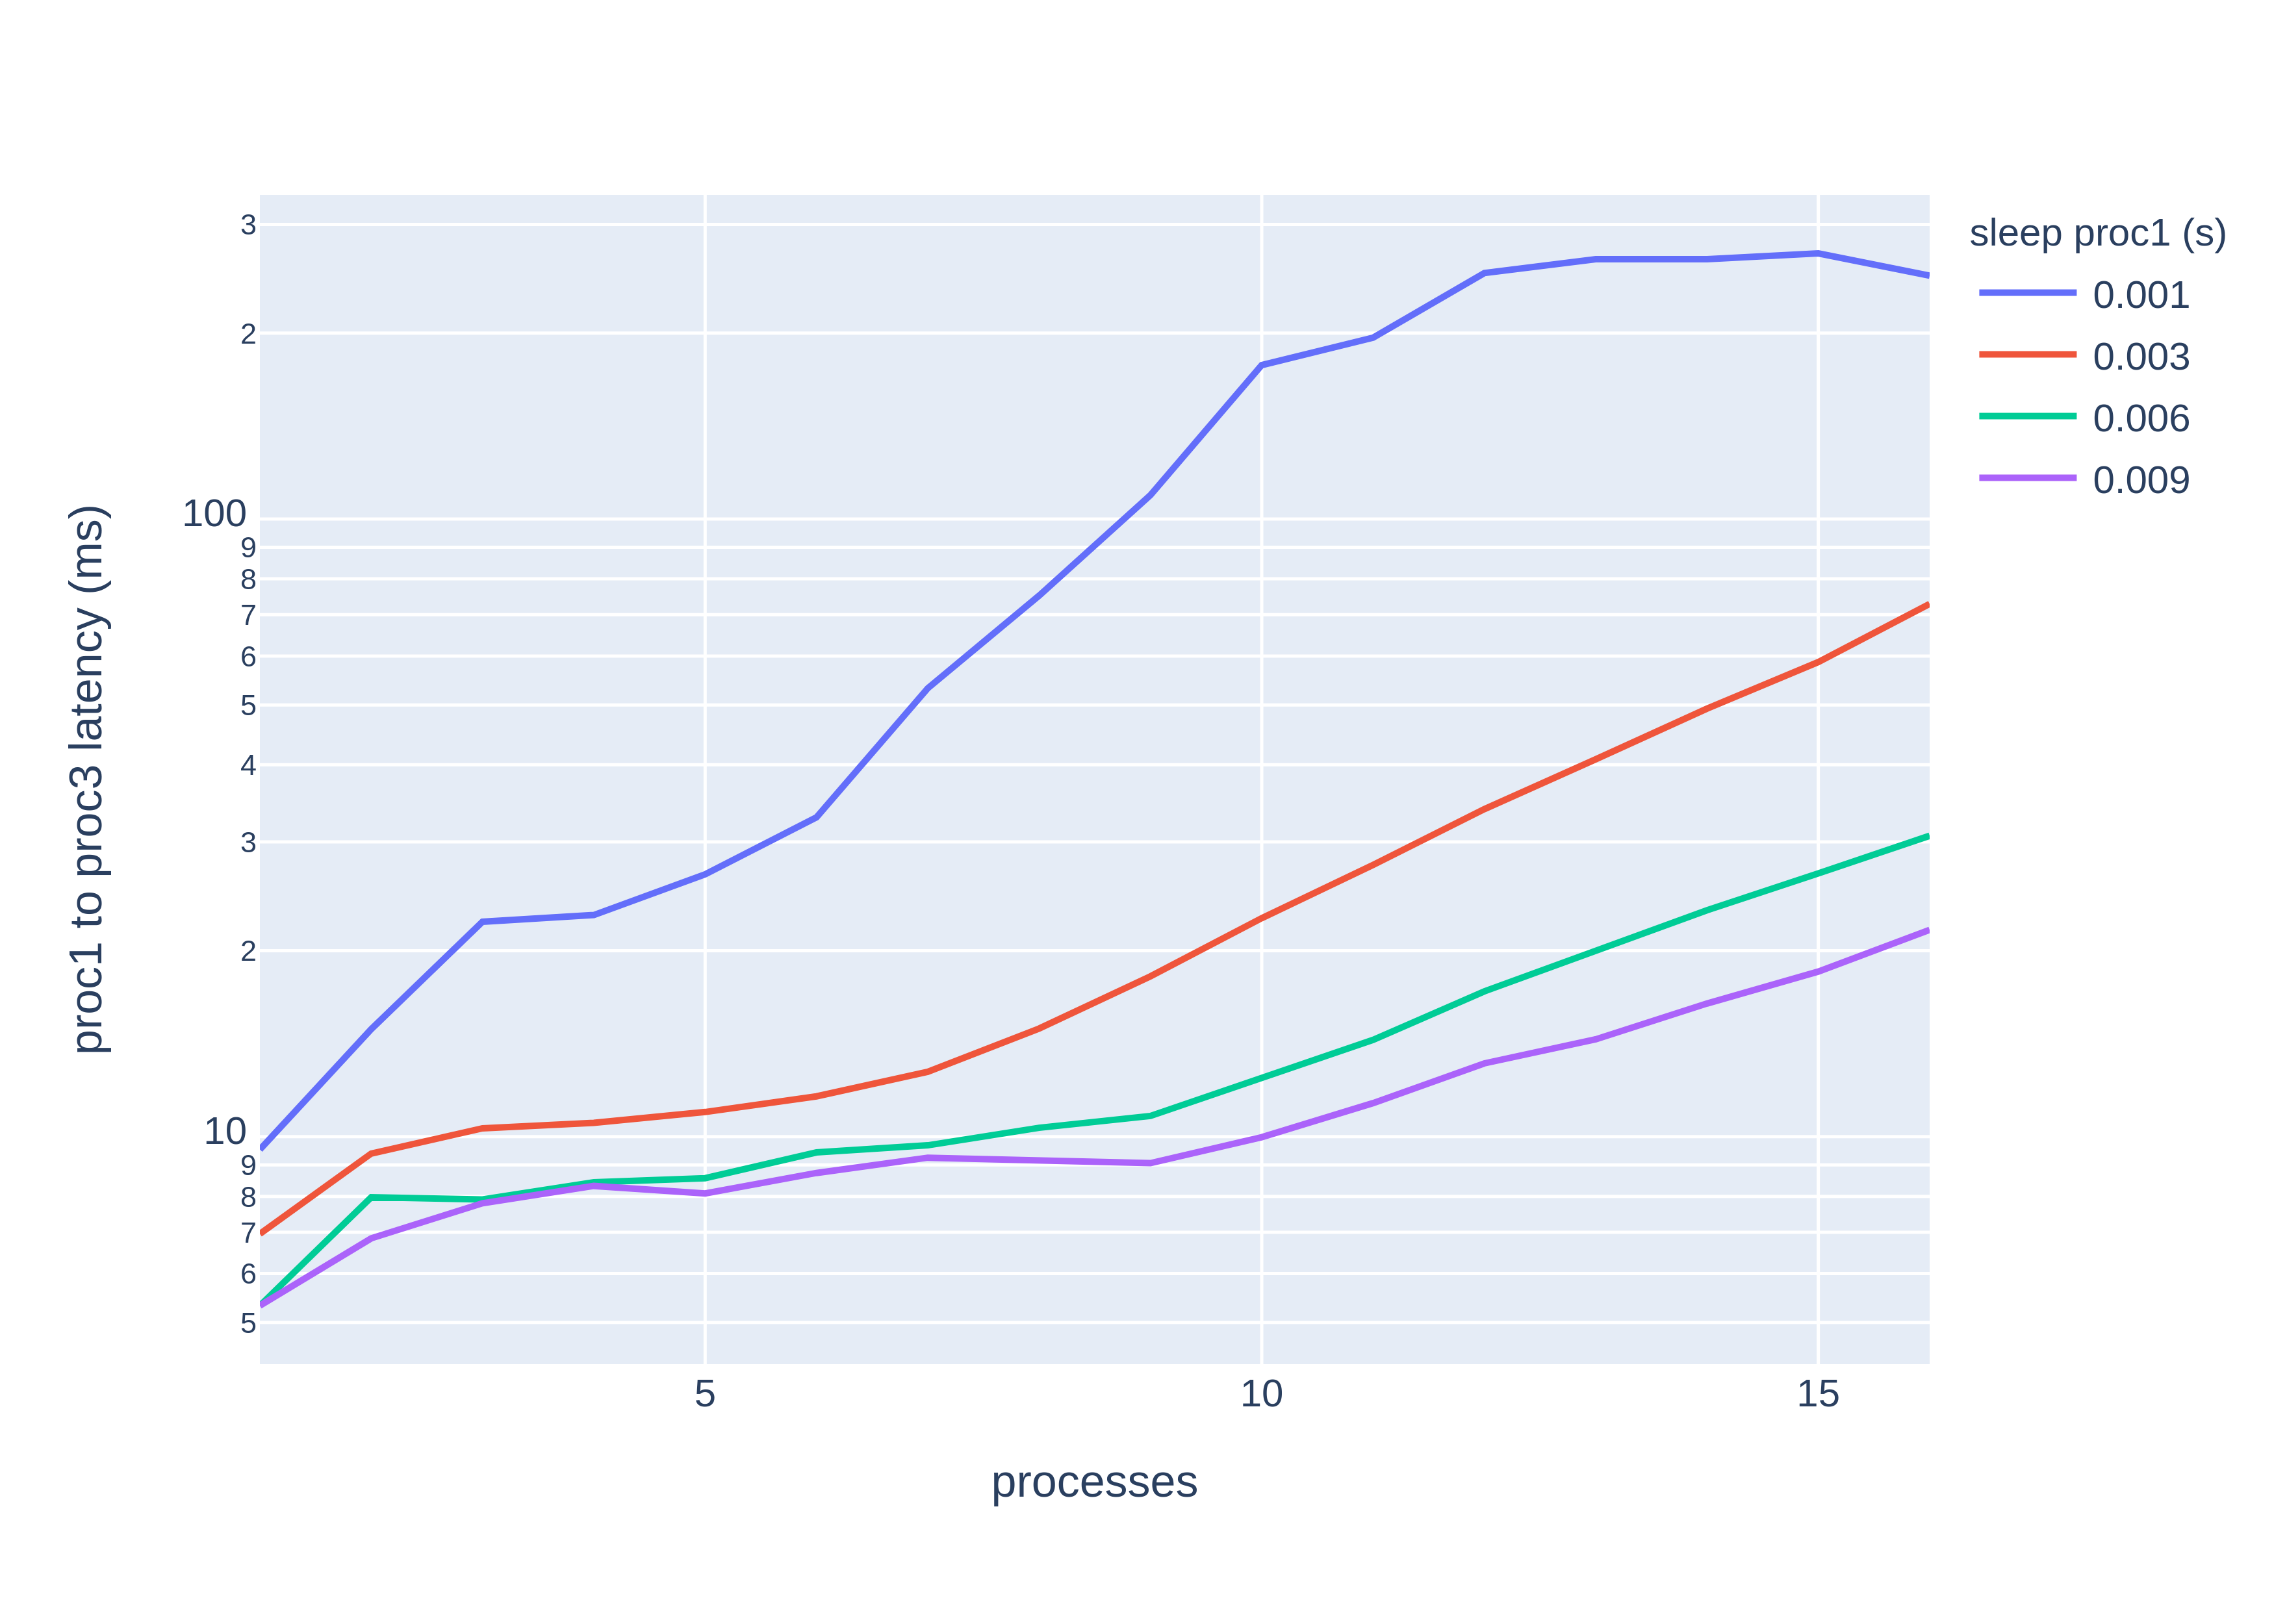
\includegraphics[width=0.9\textwidth]{./graphs/diff_in_end_postgres_all_sleeps.png}
%     \caption{Średni czas obsługi reklamy dla postgresa}
% \end{figure}


% \begin{figure}[H]
%     \centering
%     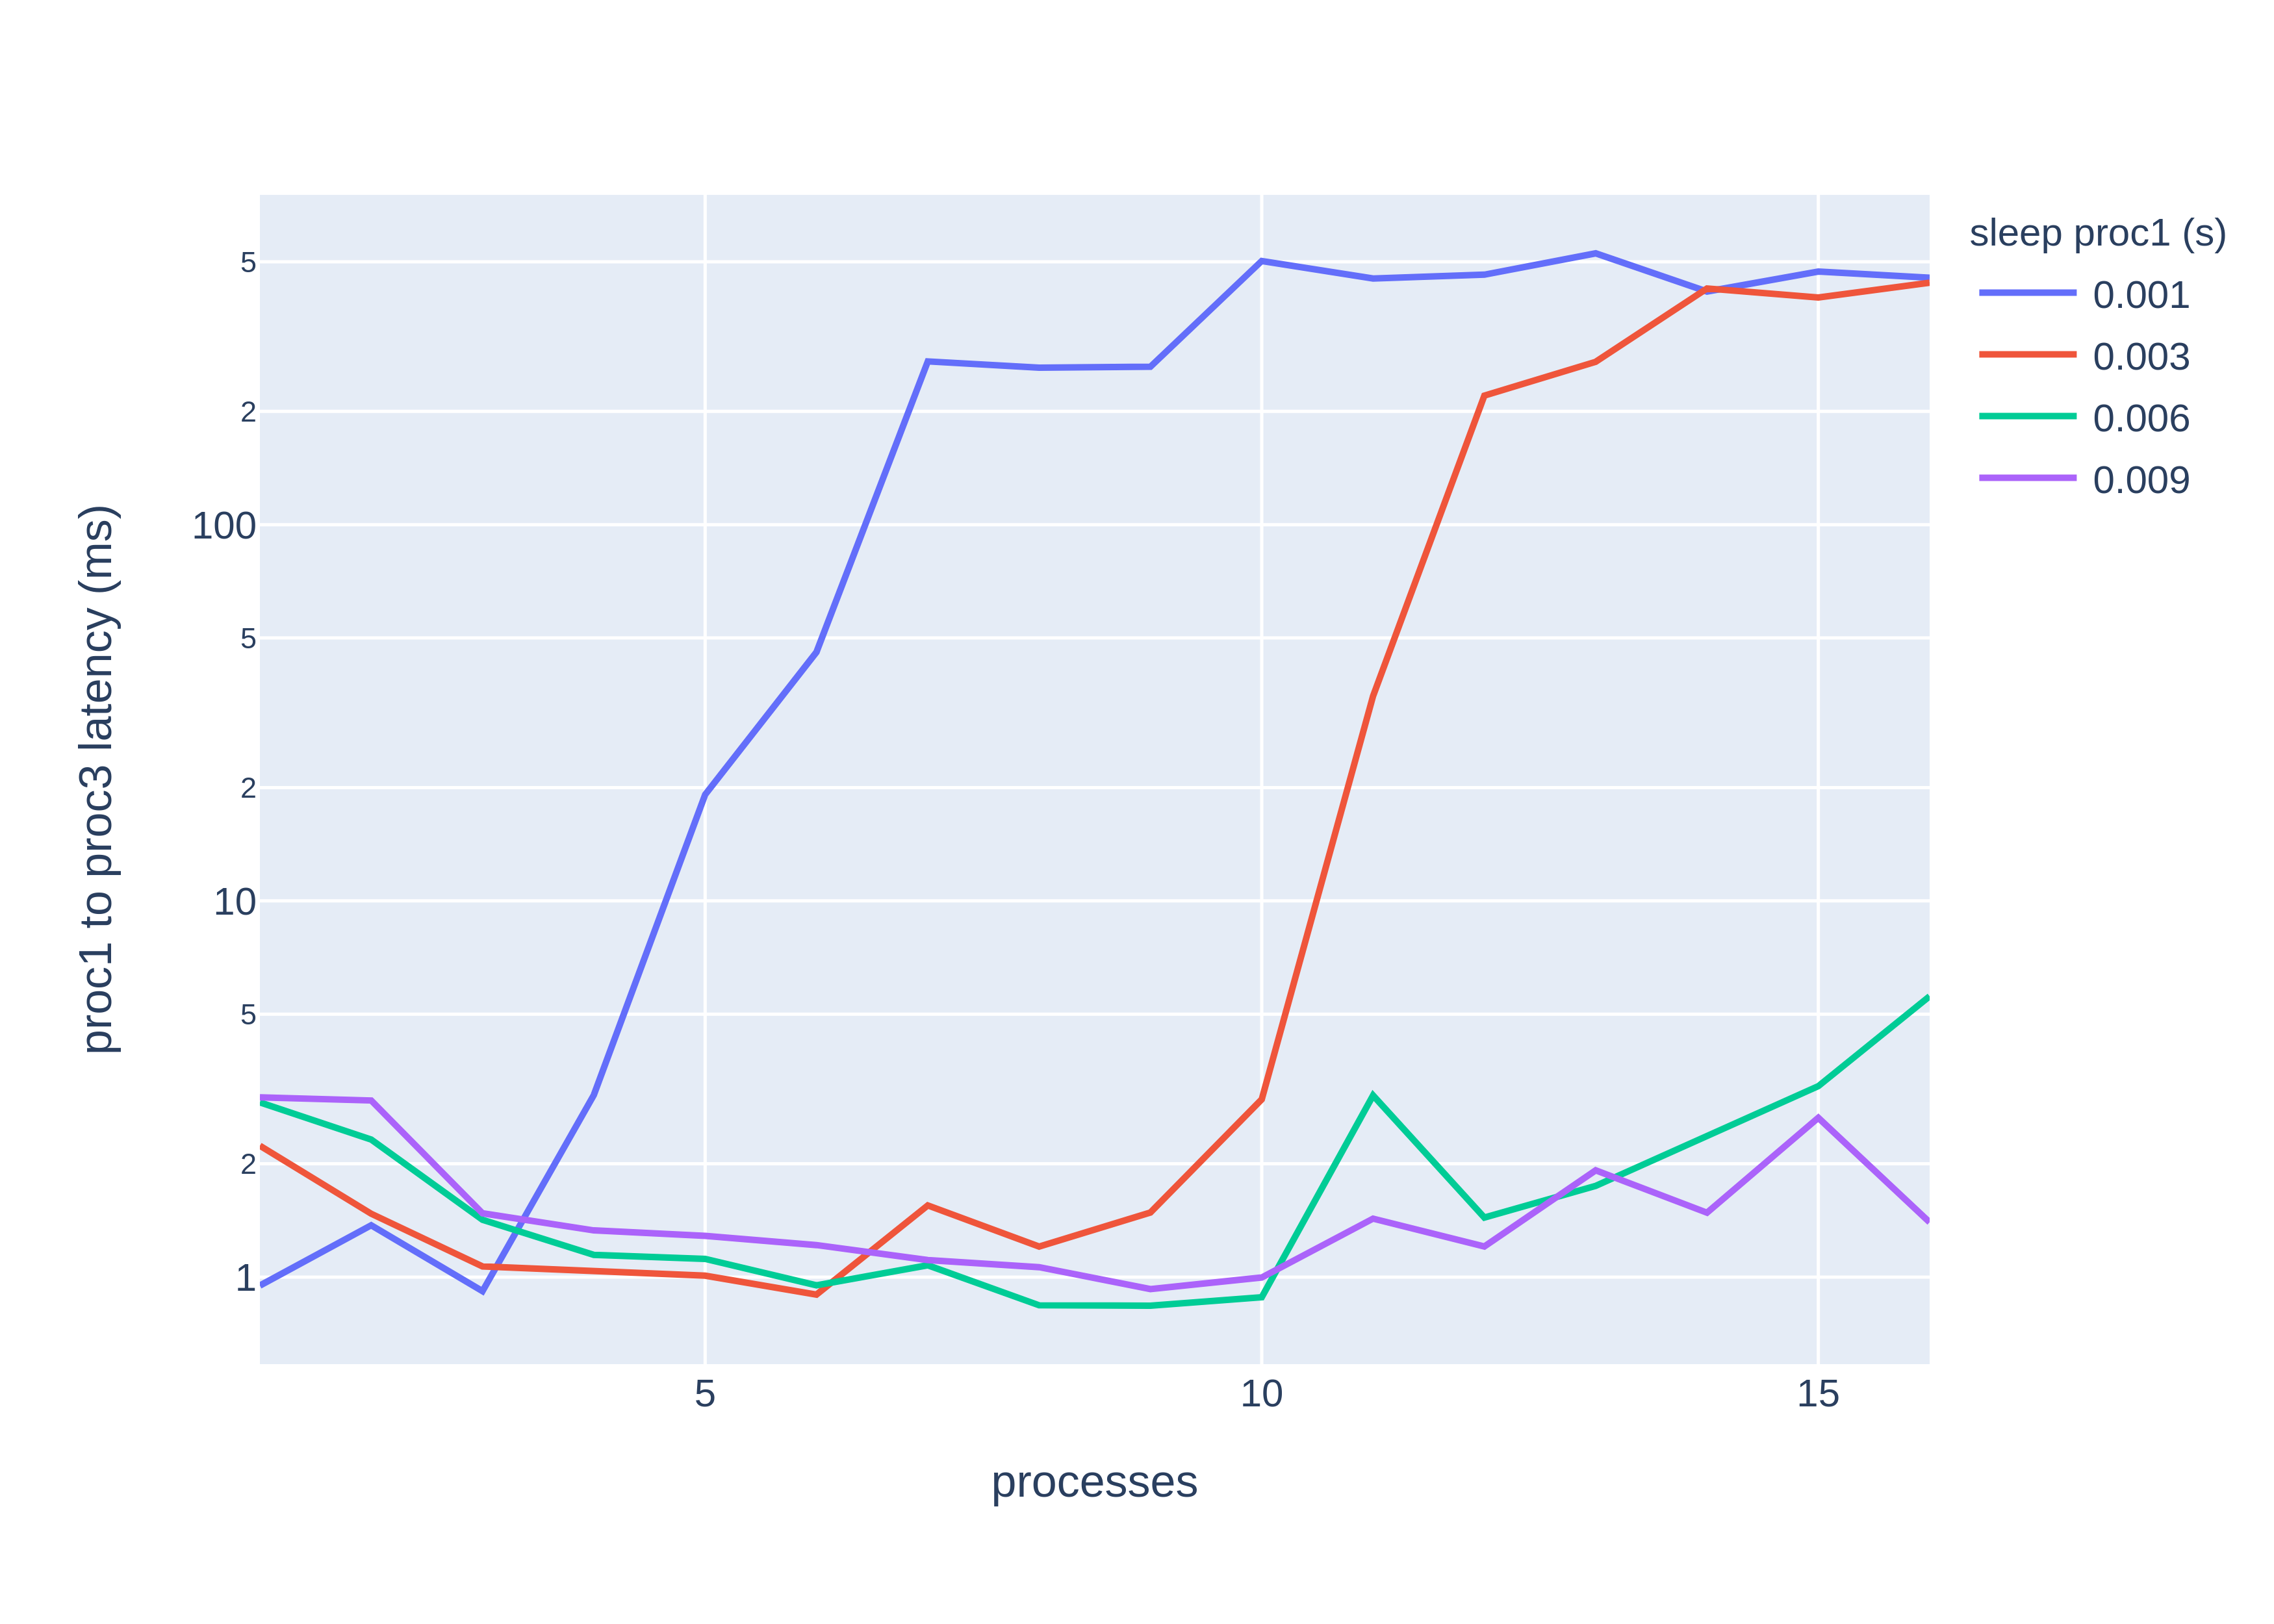
\includegraphics[width=0.9\textwidth]{./graphs/diff_in_end_redis_all_sleeps.png}
%     \caption{Średni czas obsługi reklamy dla redisa}
% \end{figure}

\begin{figure}[H]
    \centering
    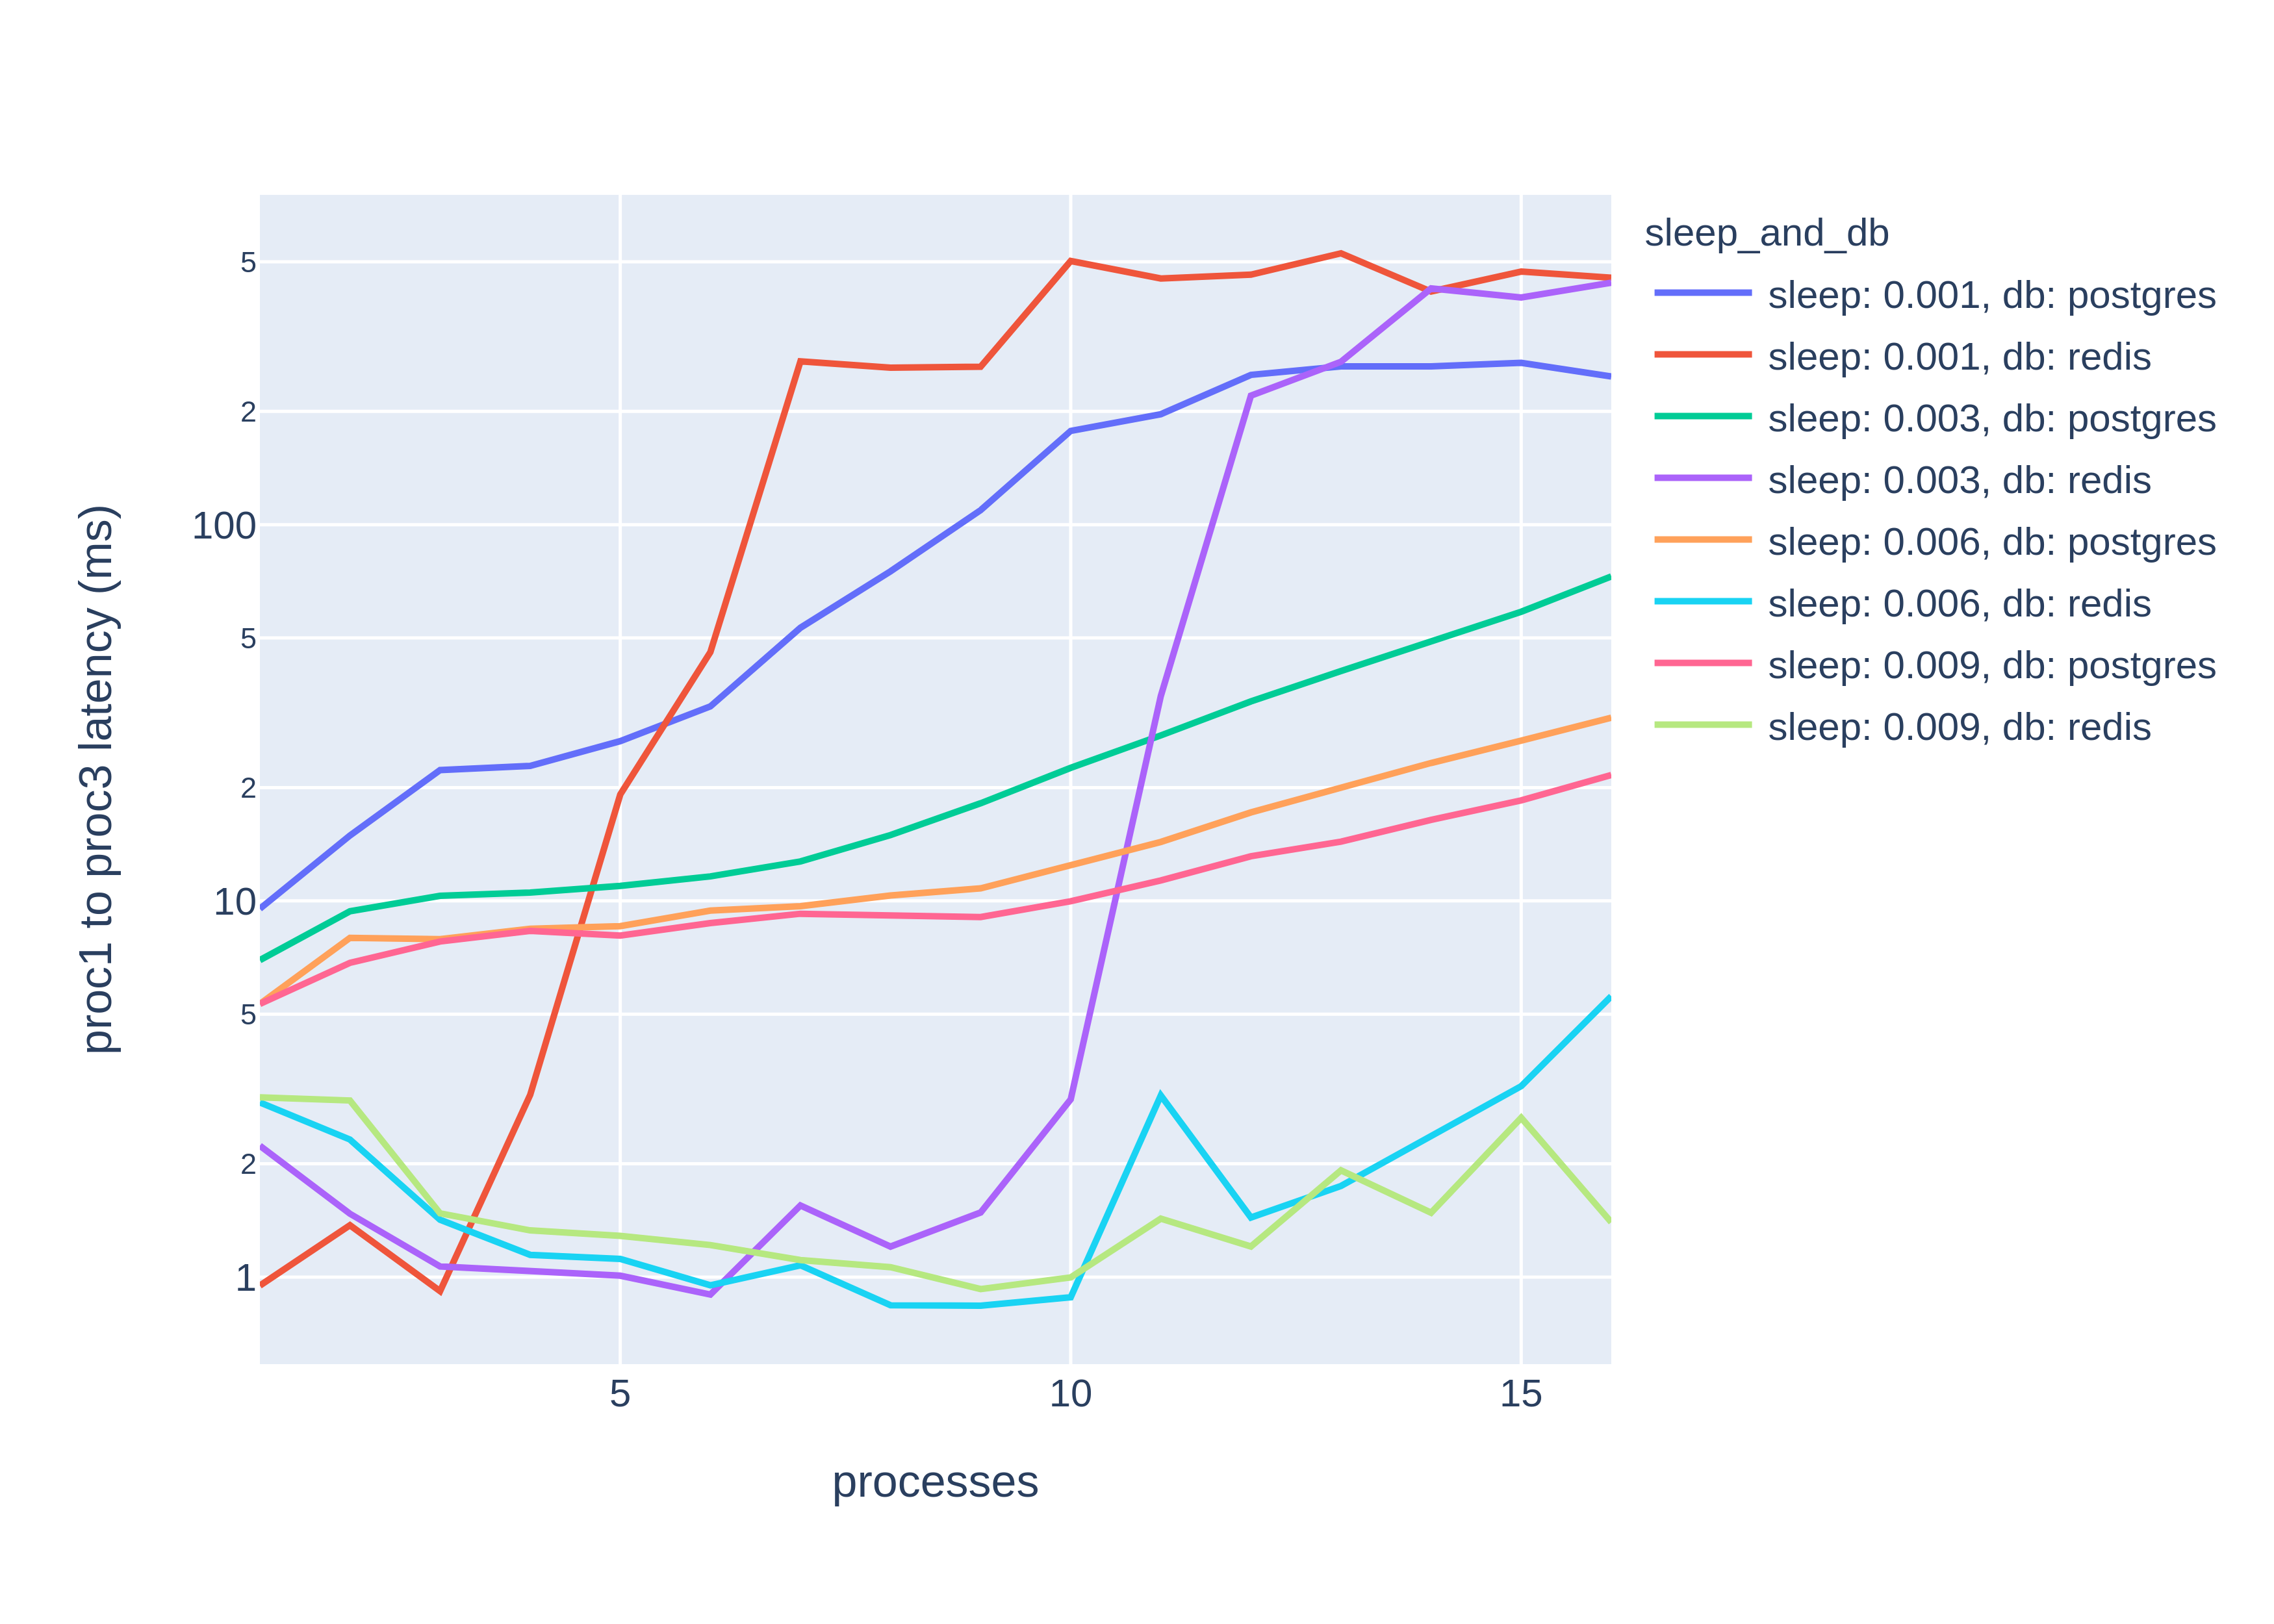
\includegraphics[width=0.9\textwidth]{./graphs/diff_in_end_all_sleeps.png}
    \caption{Średni czas obsługi reklamy}
\end{figure}

Wzrost czasu wykonania w zależności od liczby procesów jest dosyć wolny i stabilny w przypadku postgresa.

Wzrost czasu wykonania w zależności od liczby procesów jest dużo bardziej gwałtowny jeżeli używamy redisa. Jak widać na wykresie czasy obsługi reklamy są dosyć stabilne, do pewnego momentu, potem opóźnienie eksploduje. Warto zauważyć, ze przed punktem degradacji wydajności, obsługa reklamy przez redisa zajmuje mniej niż 5ms, natomiast dla postgresa są to liczby nieosiągalne przy żadnym ustawieniu.

\begin{figure}[H]
    \centering
    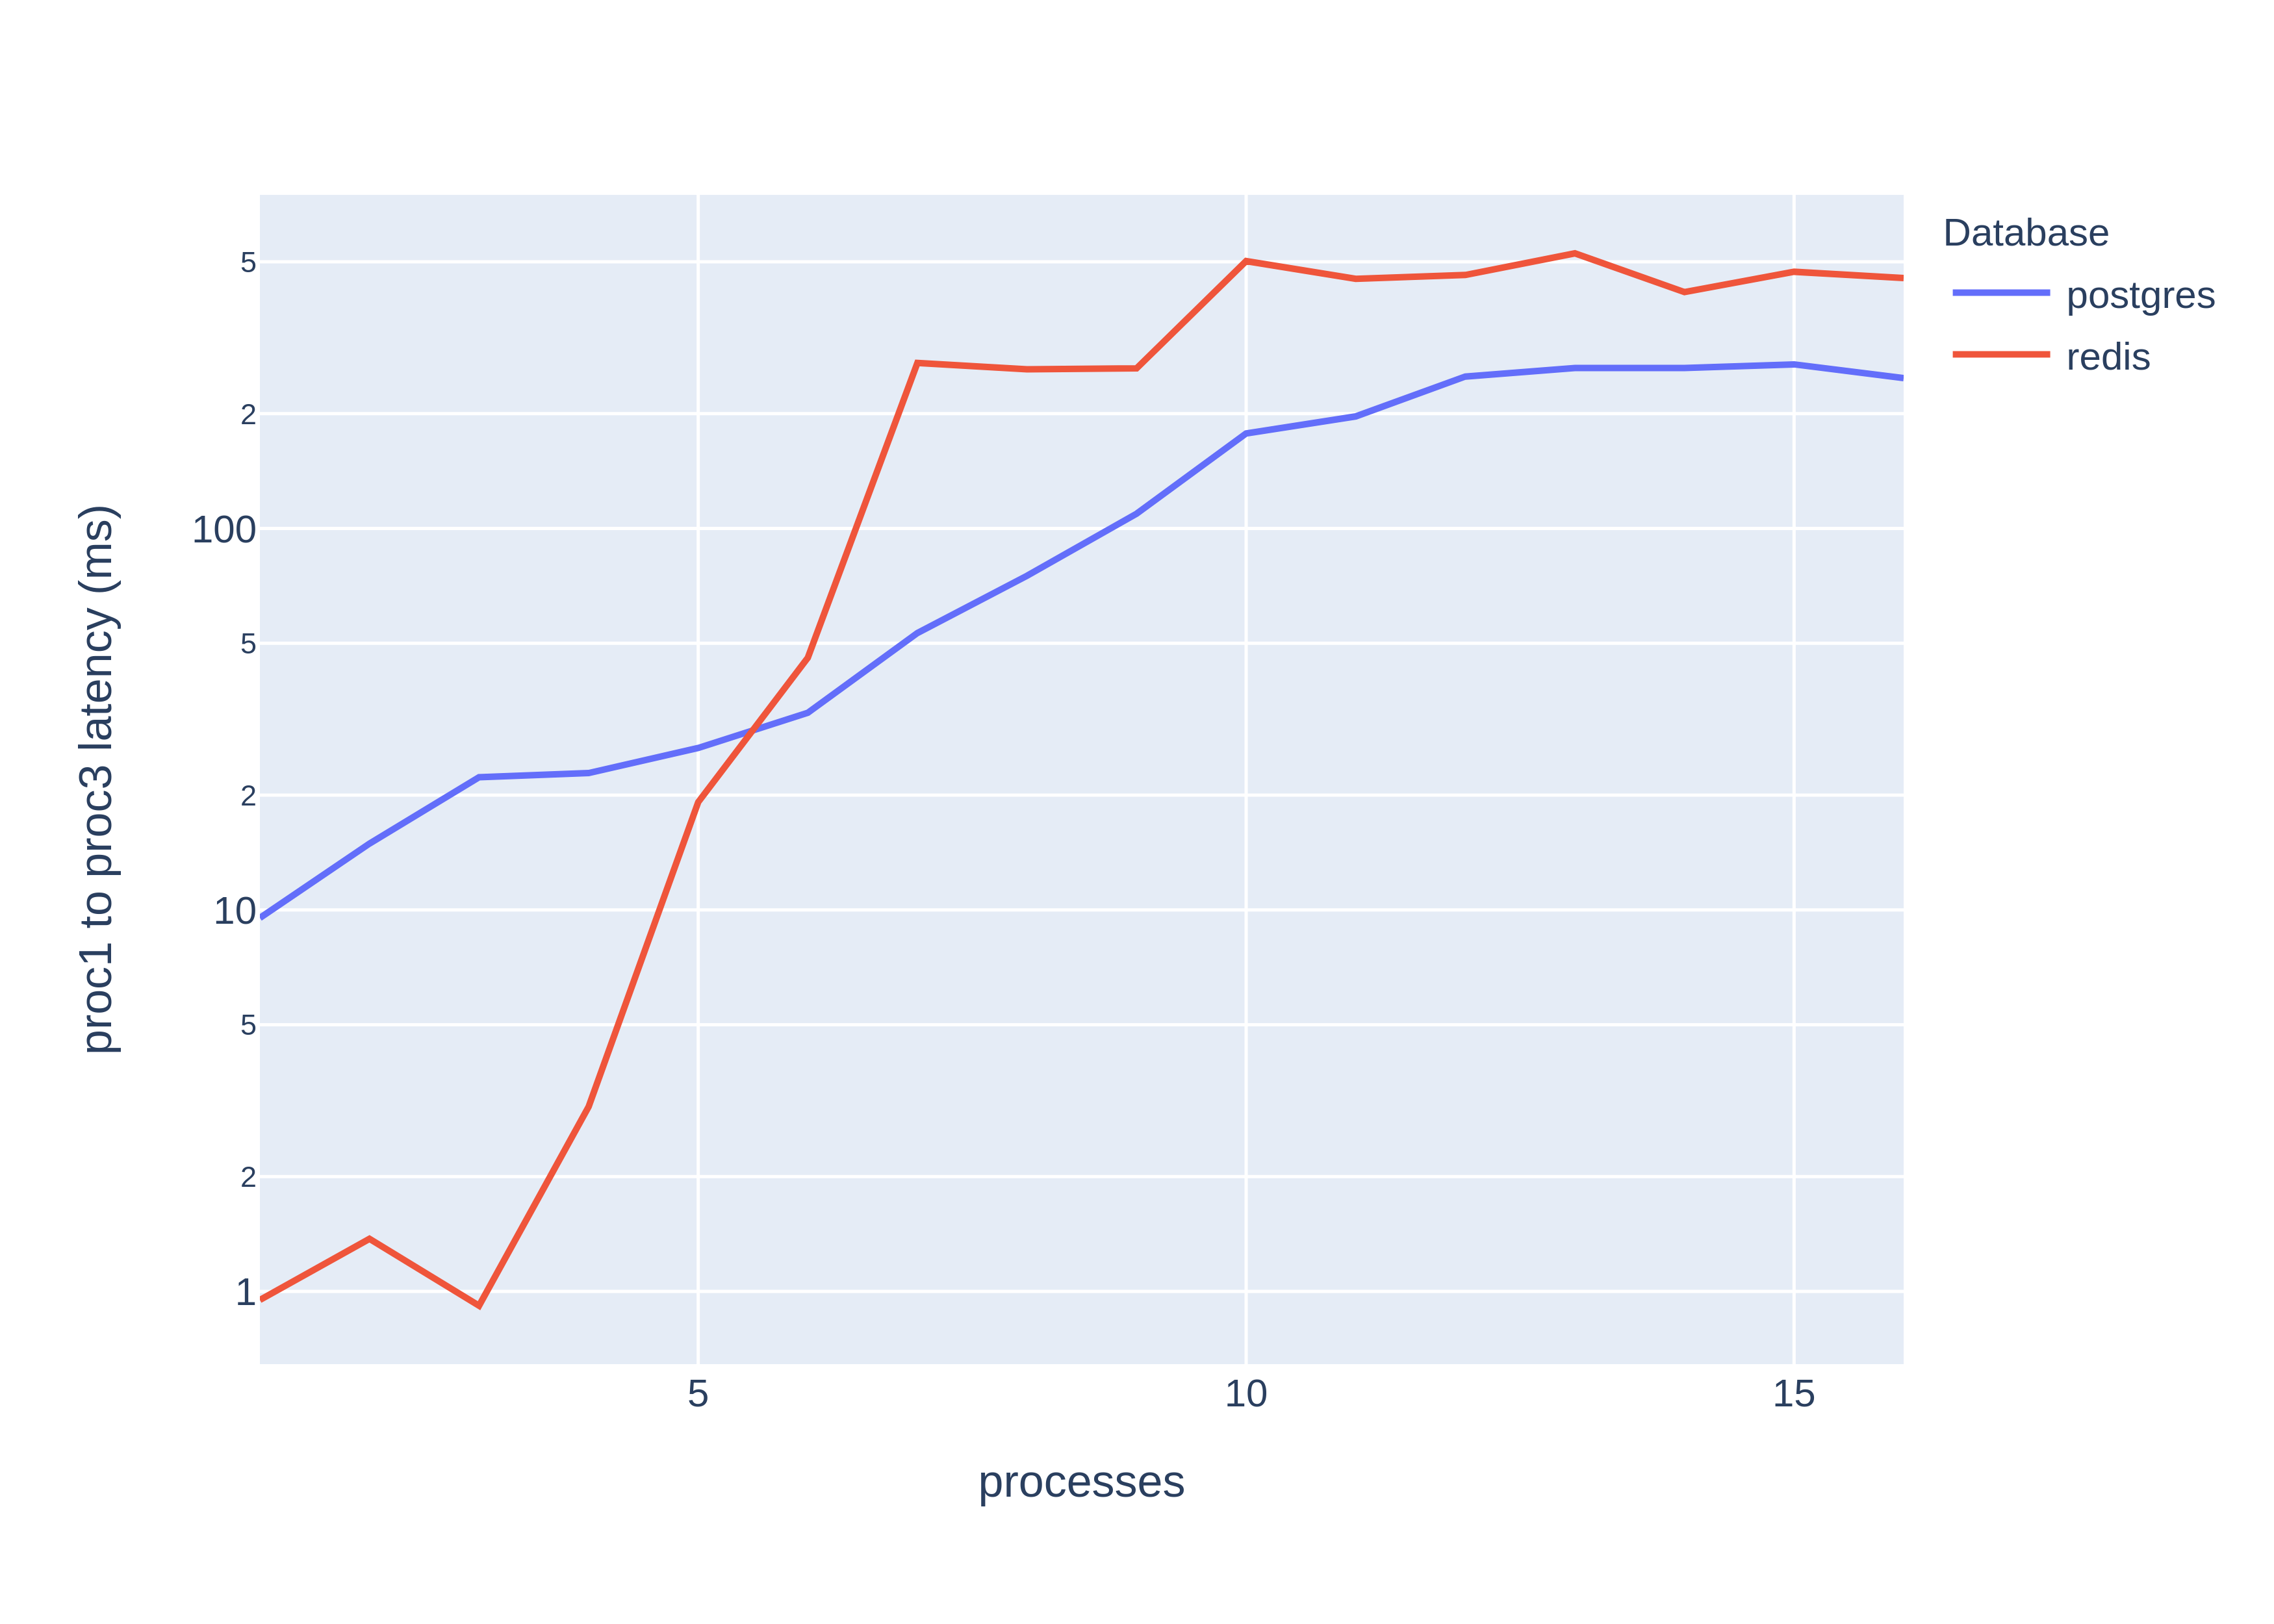
\includegraphics[width=0.9\textwidth]{./graphs/diff_in_end_postgres_vs_redis0001.png}
    \caption{Porównanie średniego czasu obsługi reklamy w zależności od bazy danych dla t=0.001}
\end{figure}

\begin{figure}[H]
    \centering
    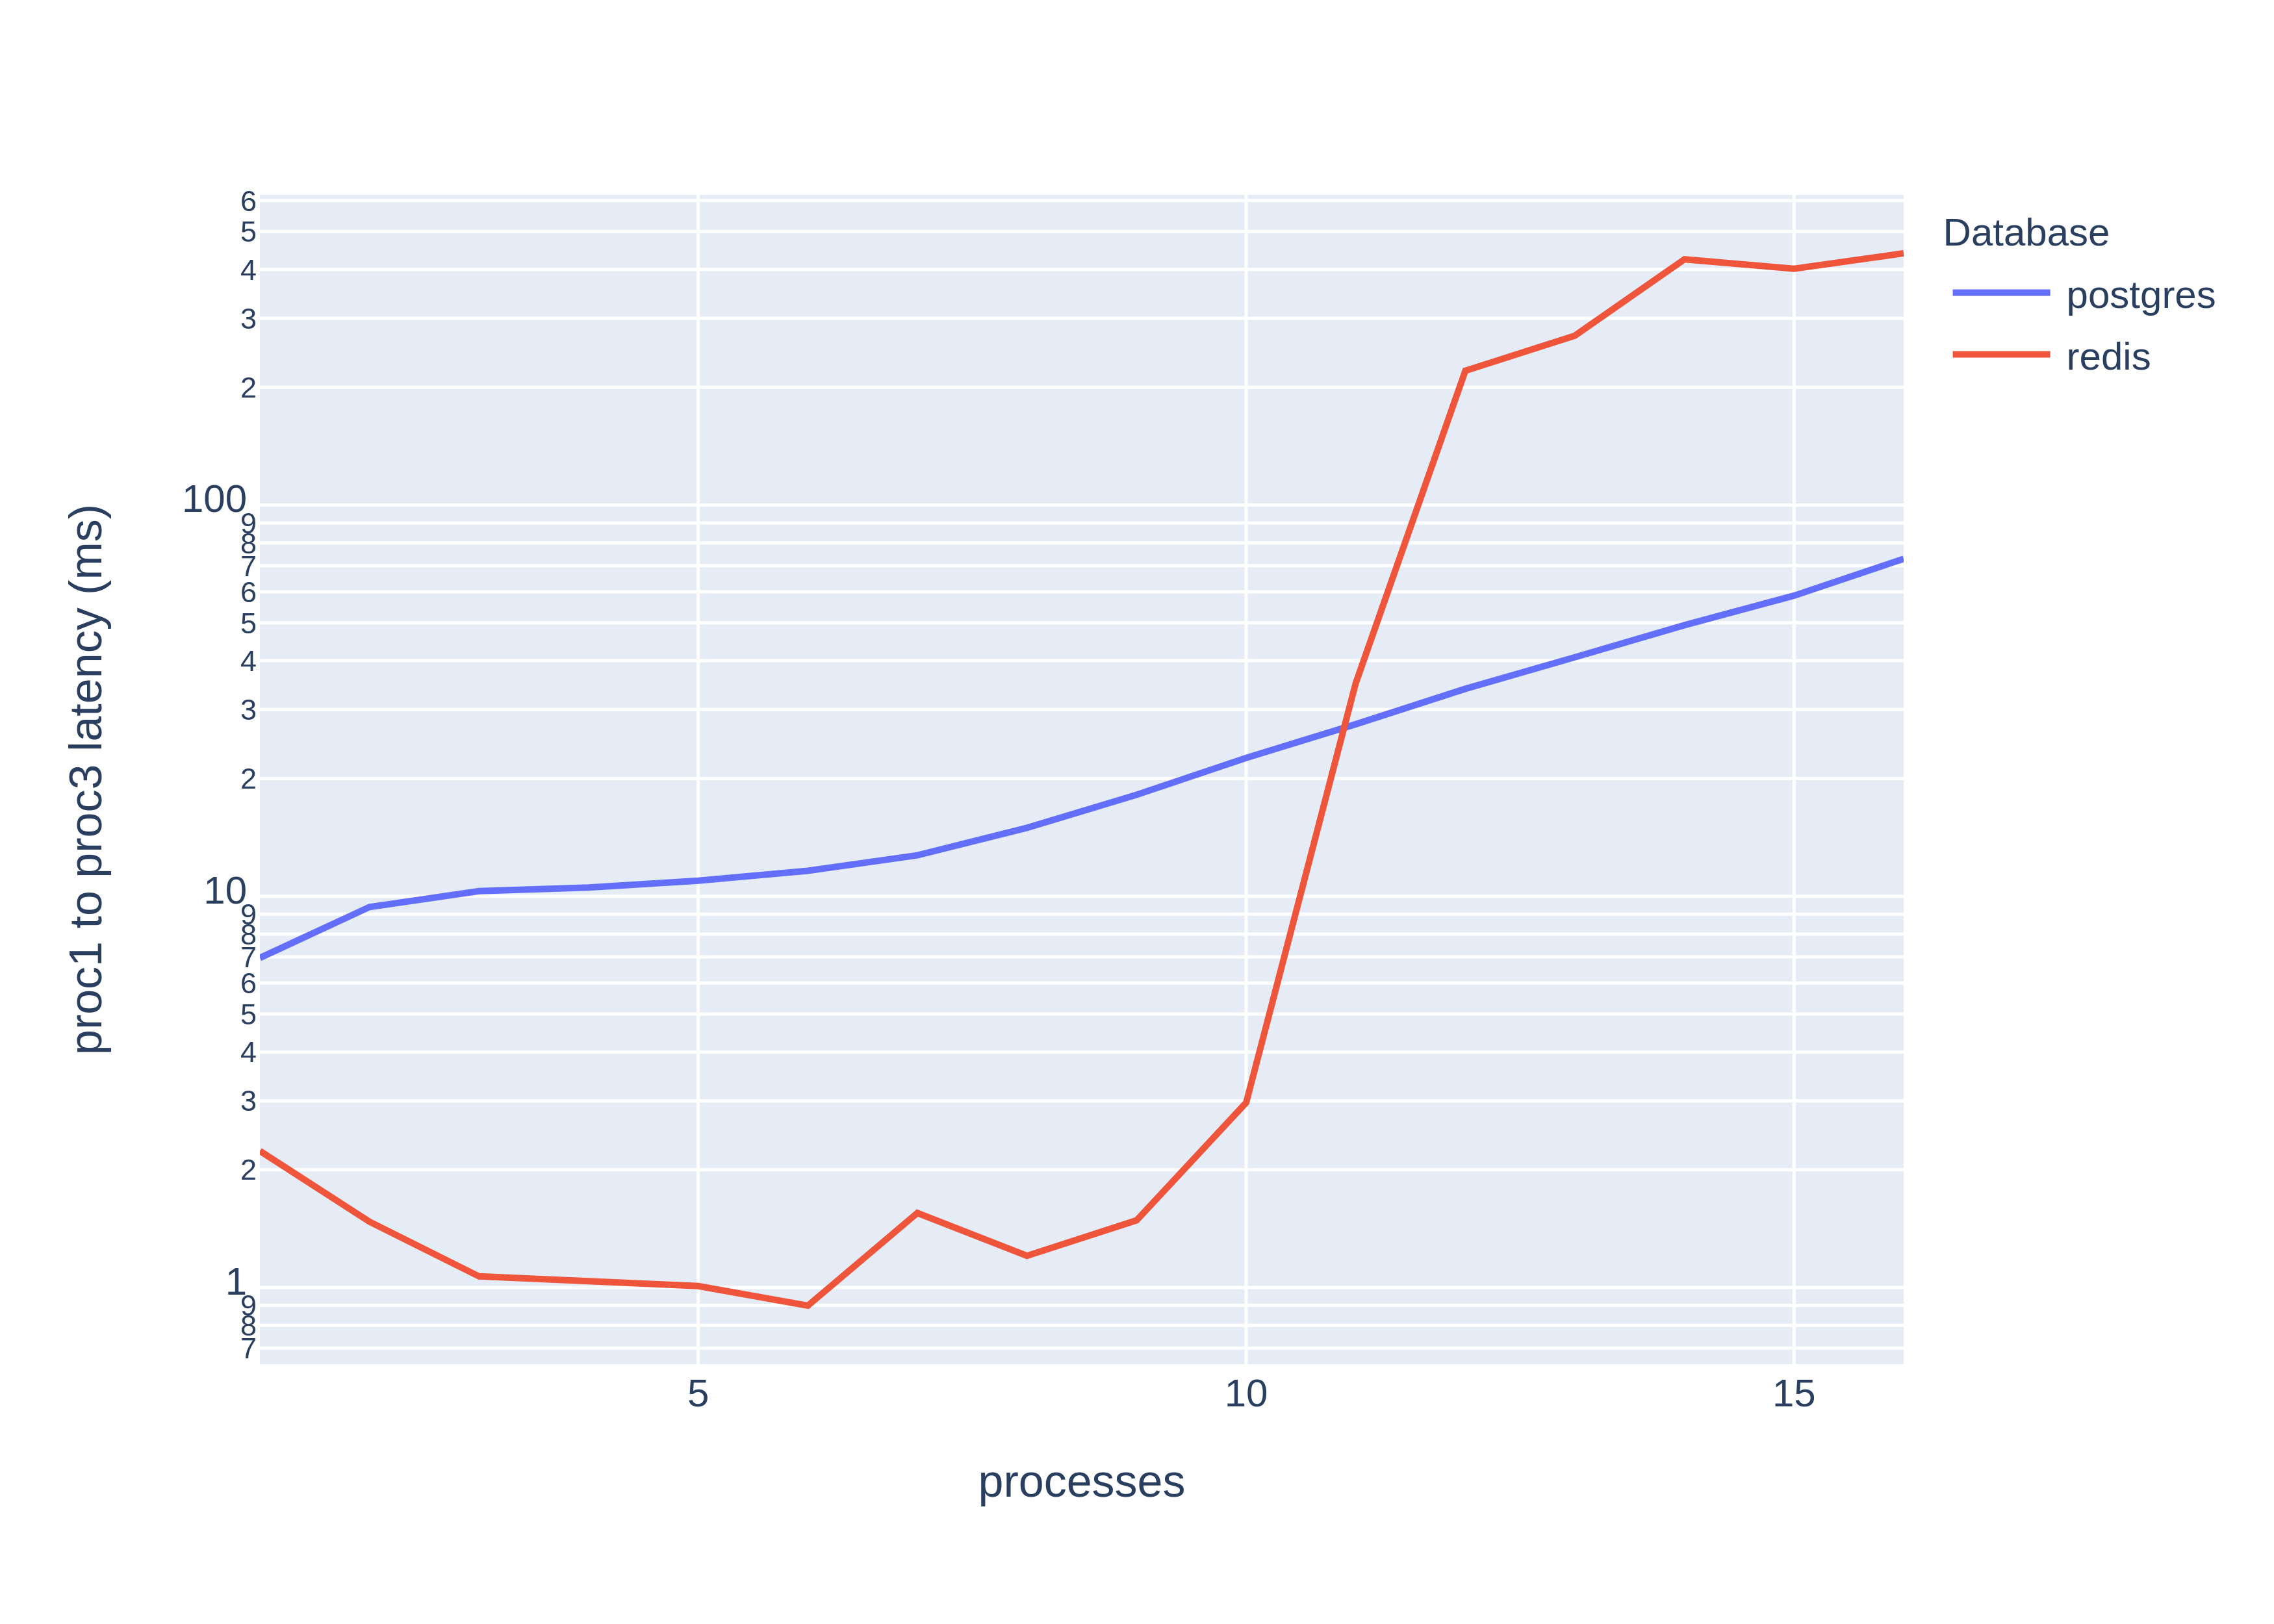
\includegraphics[width=0.9\textwidth]{./graphs/diff_in_end_postgres_vs_redis0003.png}
    \caption{Porównanie średniego czasu obsługi reklamy w zależności od bazy danych dla t=0.003}
\end{figure}

\begin{figure}[H]
    \centering
    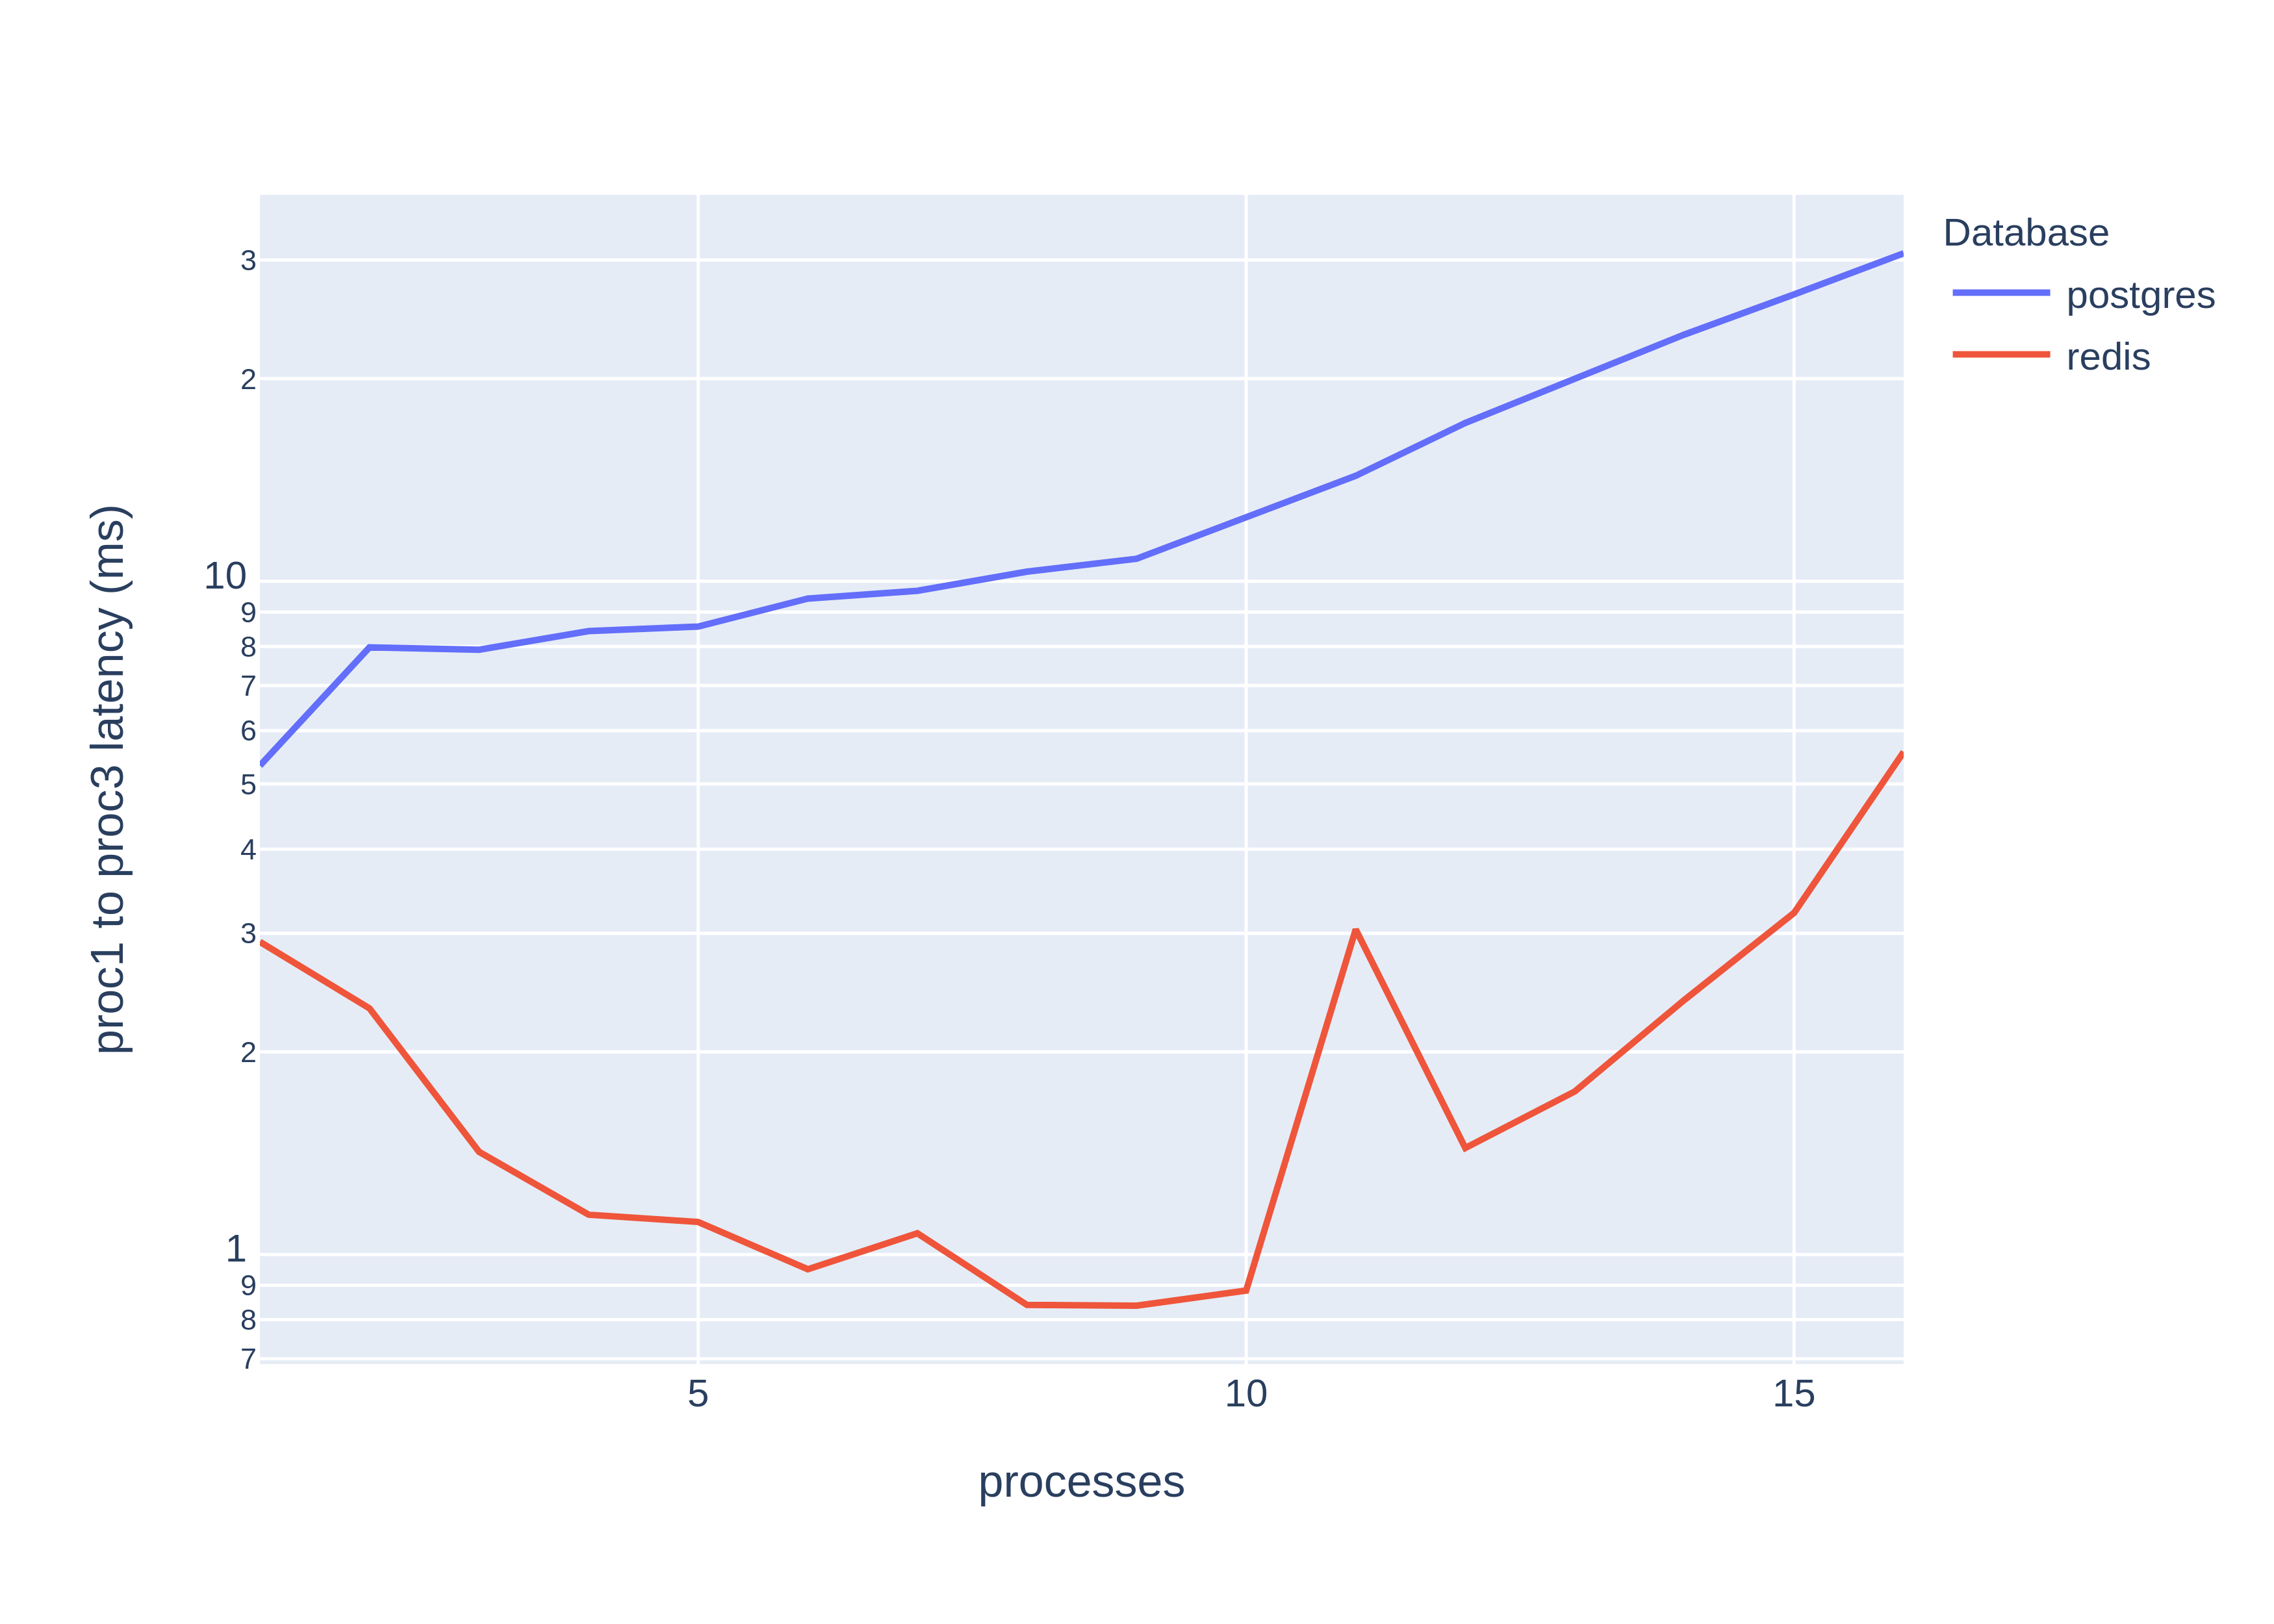
\includegraphics[width=0.9\textwidth]{./graphs/diff_in_end_postgres_vs_redis0006.png}
    \caption{Porównanie średniego czasu obsługi reklamy w zależności od bazy danych dla t=0.006}
\end{figure}

\begin{figure}[H]
    \centering
    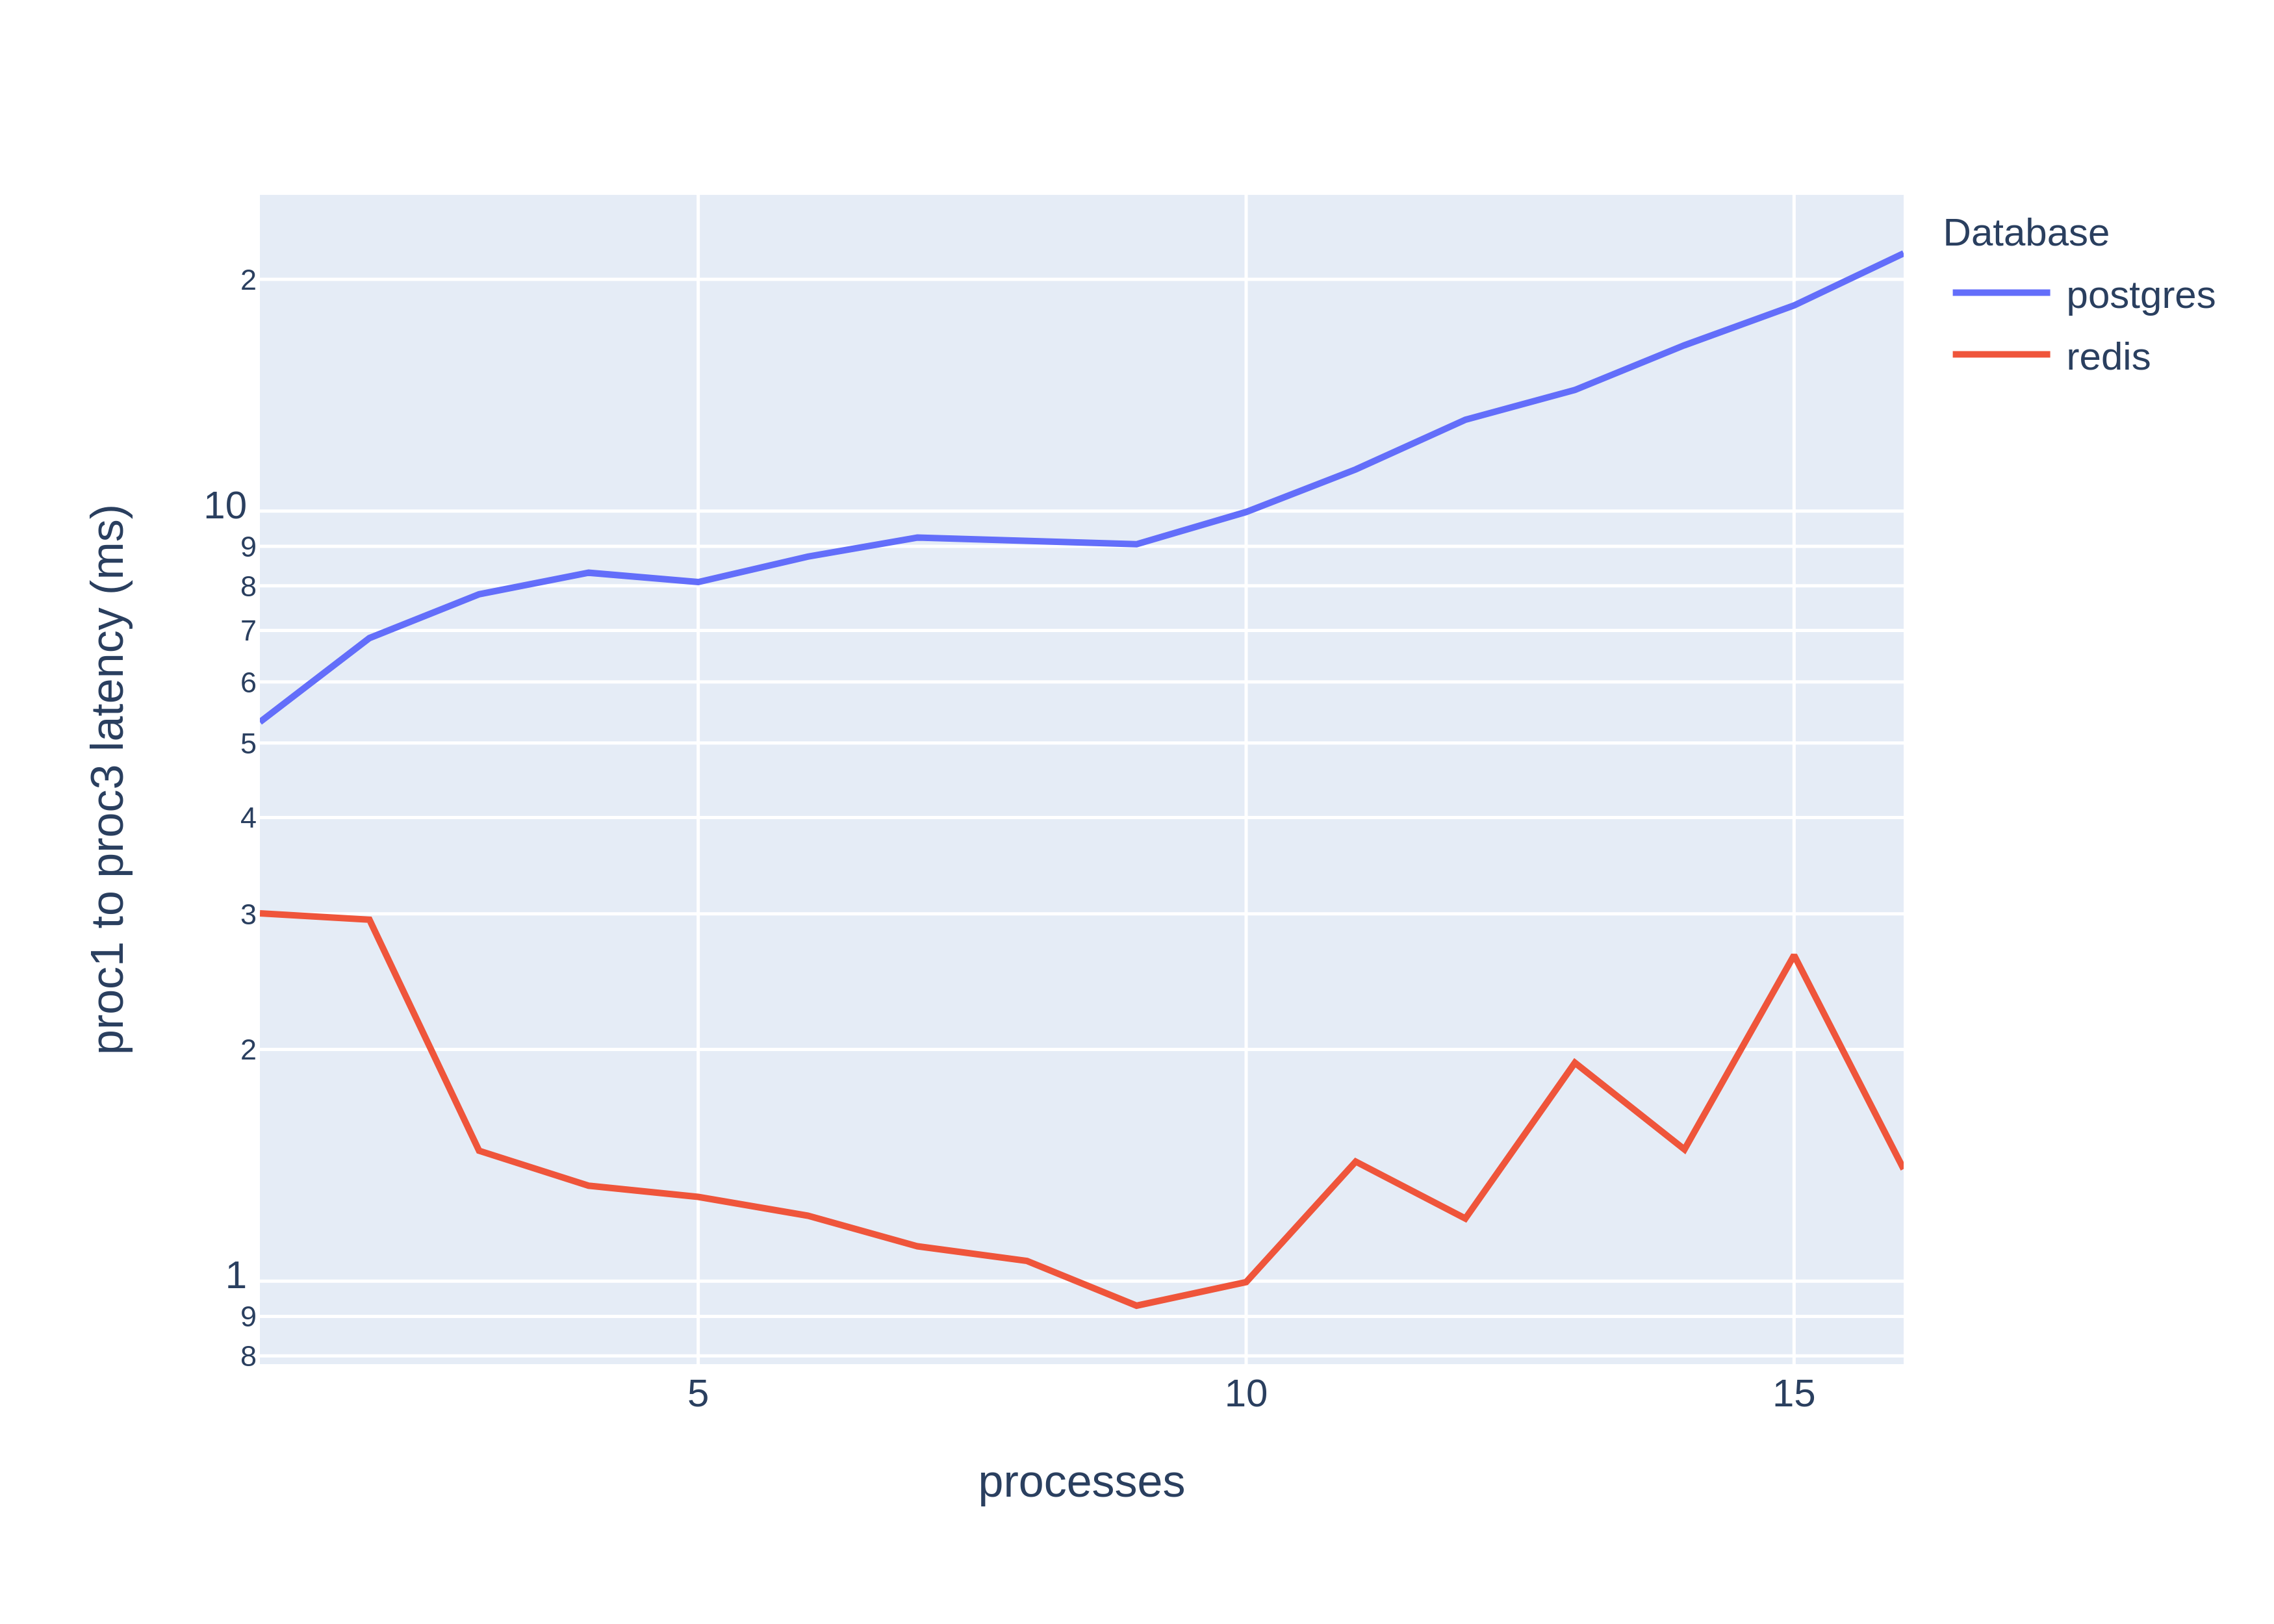
\includegraphics[width=0.9\textwidth]{./graphs/diff_in_end_postgres_vs_redis0009.png}
    \caption{Porównanie średniego czasu obsługi reklamy w zależności od bazy danych dla t=0.009}
\end{figure}

Redis zazwyczaj jest dużo szybszą bazą niż postgres, ale kiedy obciążenie jest bardzo wysokie, to postgres oferuję szybsza obsługę reklam. Szczególnie jest to widoczne dla $t=0.001$ i $t=0.003$.


\subsection{Prawdopodobieństwo wyemitowania reklamy poniżej 20ms}

% \begin{figure}[H]
%     \centering
%     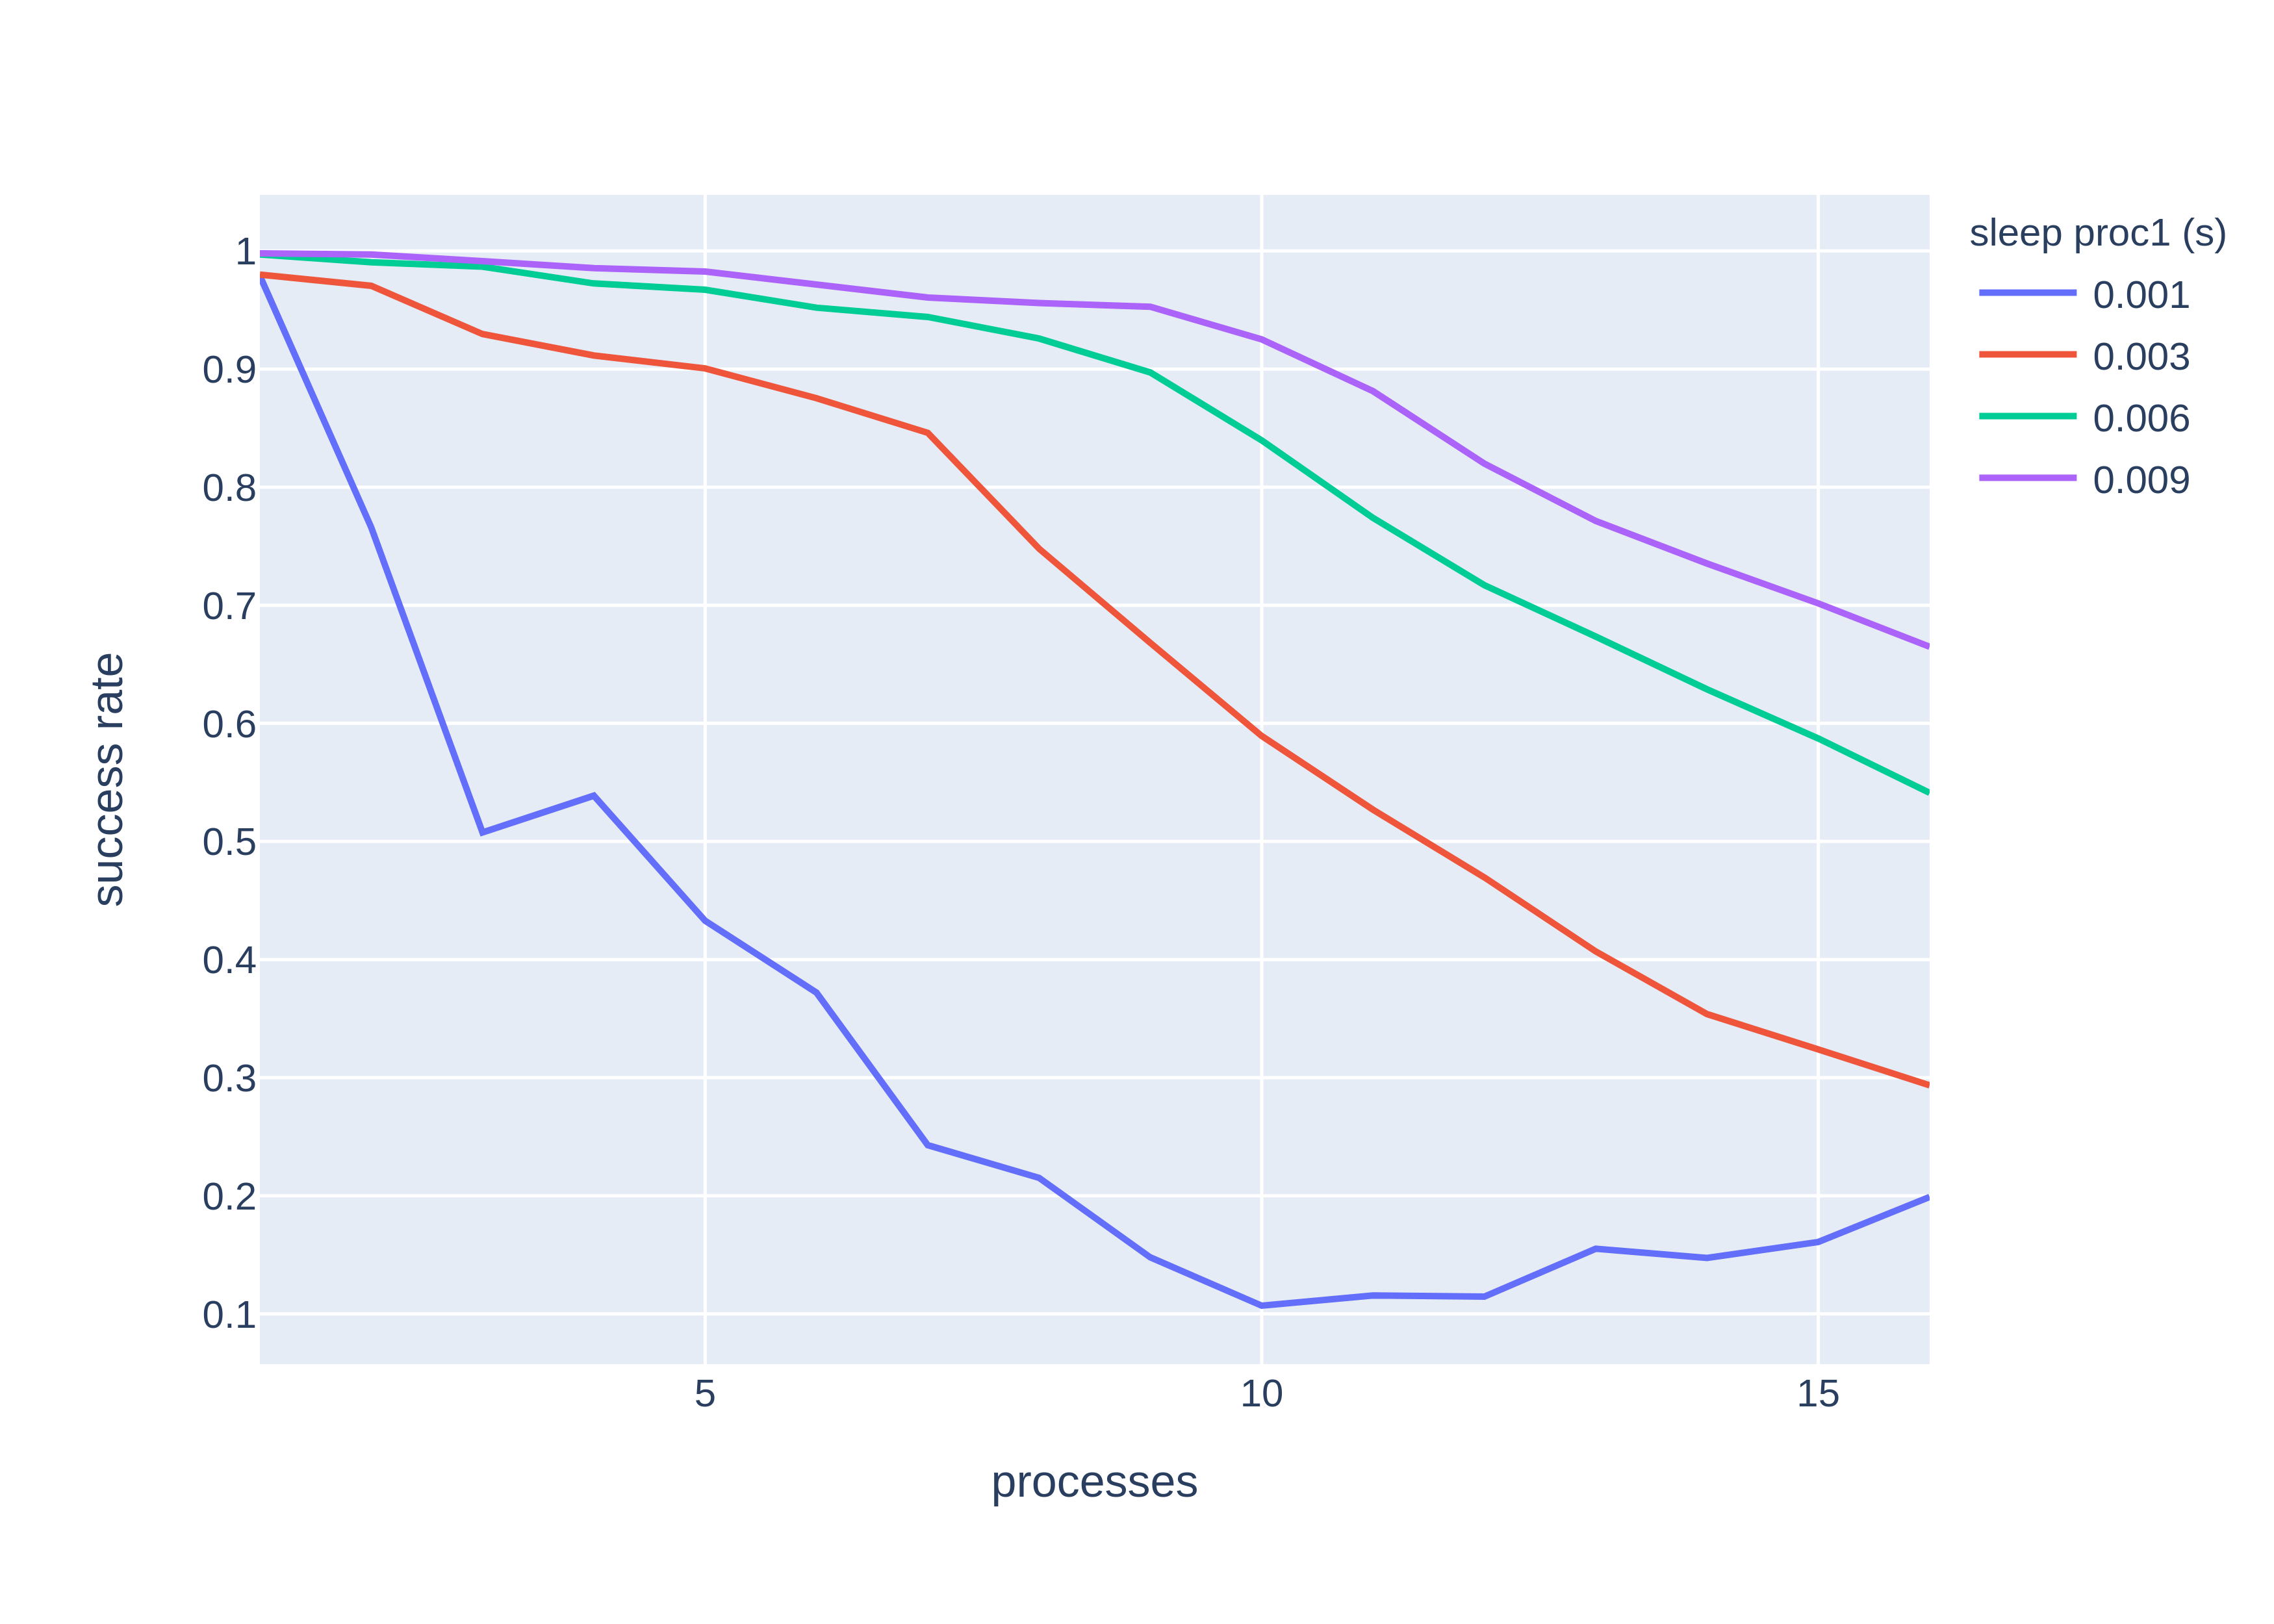
\includegraphics[width=0.9\textwidth]{./graphs/success_rate_postgres_all_sleeps.png}
%     \caption{Prawdopodobieństwo wyemitowania reklamy poniżej 20ms dla postgresa}
% \end{figure}

% \begin{figure}[H]
%     \centering
%     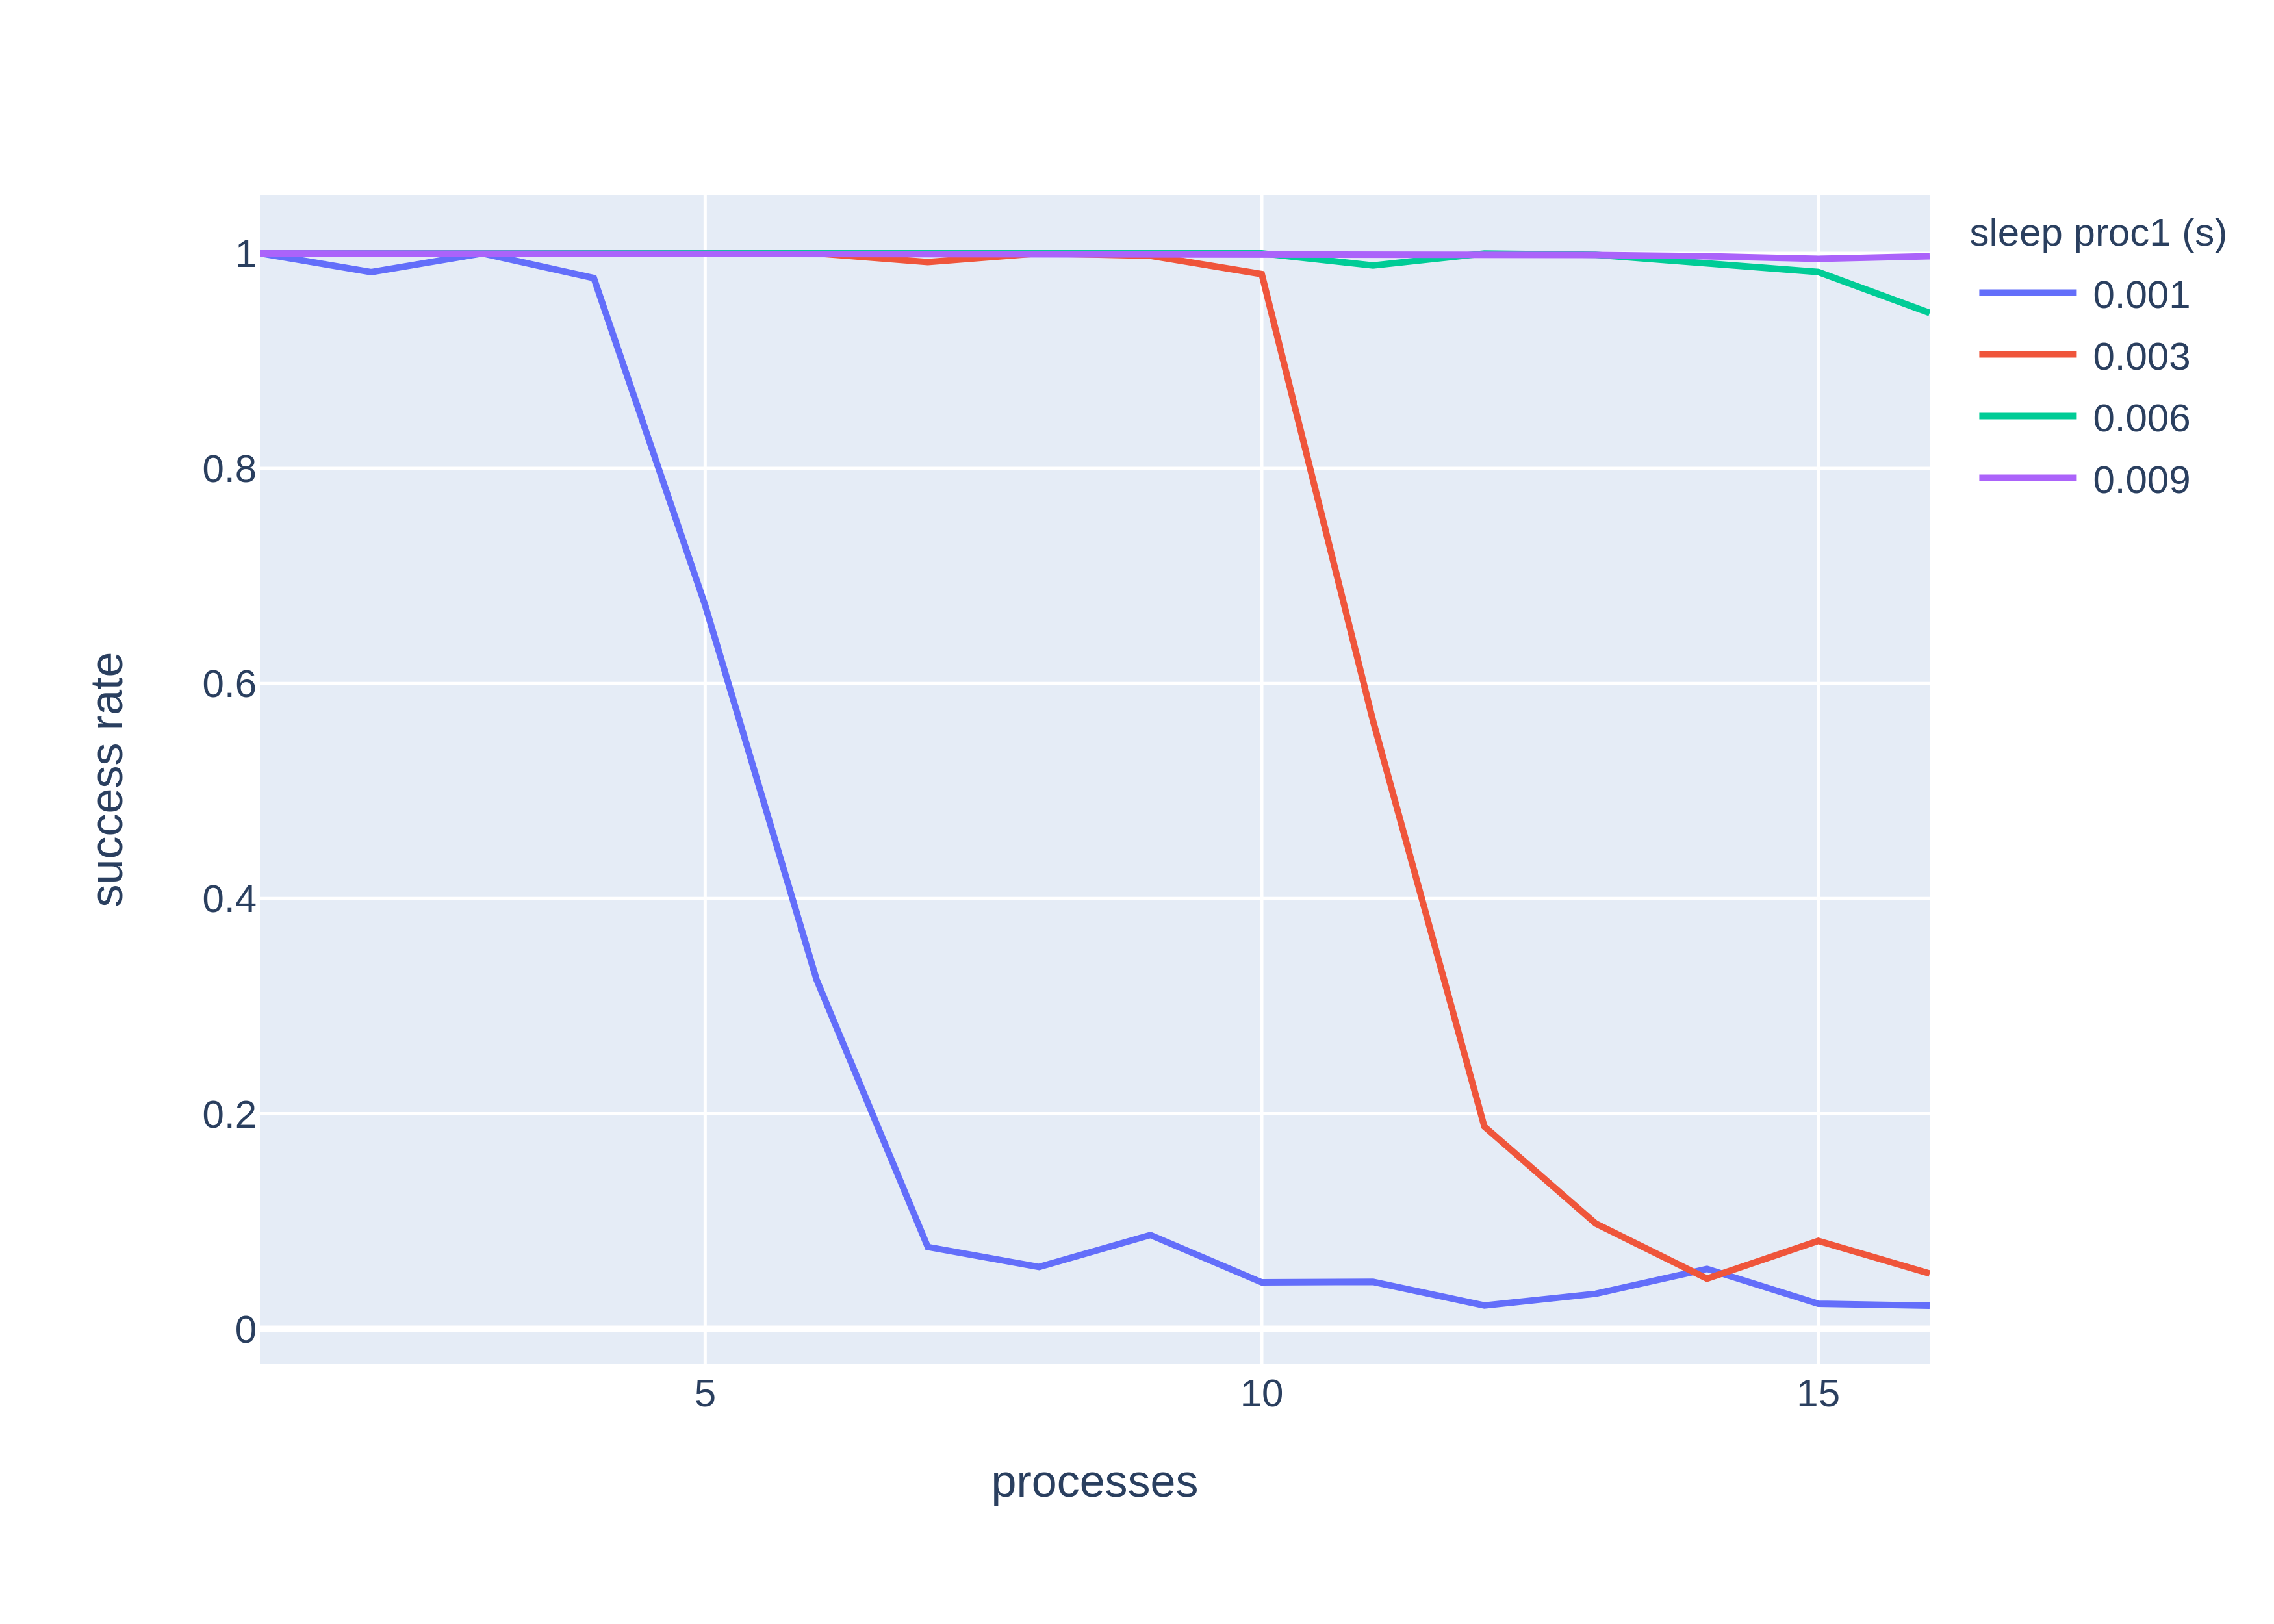
\includegraphics[width=0.9\textwidth]{./graphs/success_rate_redis_all_sleeps.png}
%     \caption{Prawdopodobieństwo wyemitowania reklamy poniżej 20ms dla redisa}
% \end{figure}

\begin{figure}[H]
    \centering
    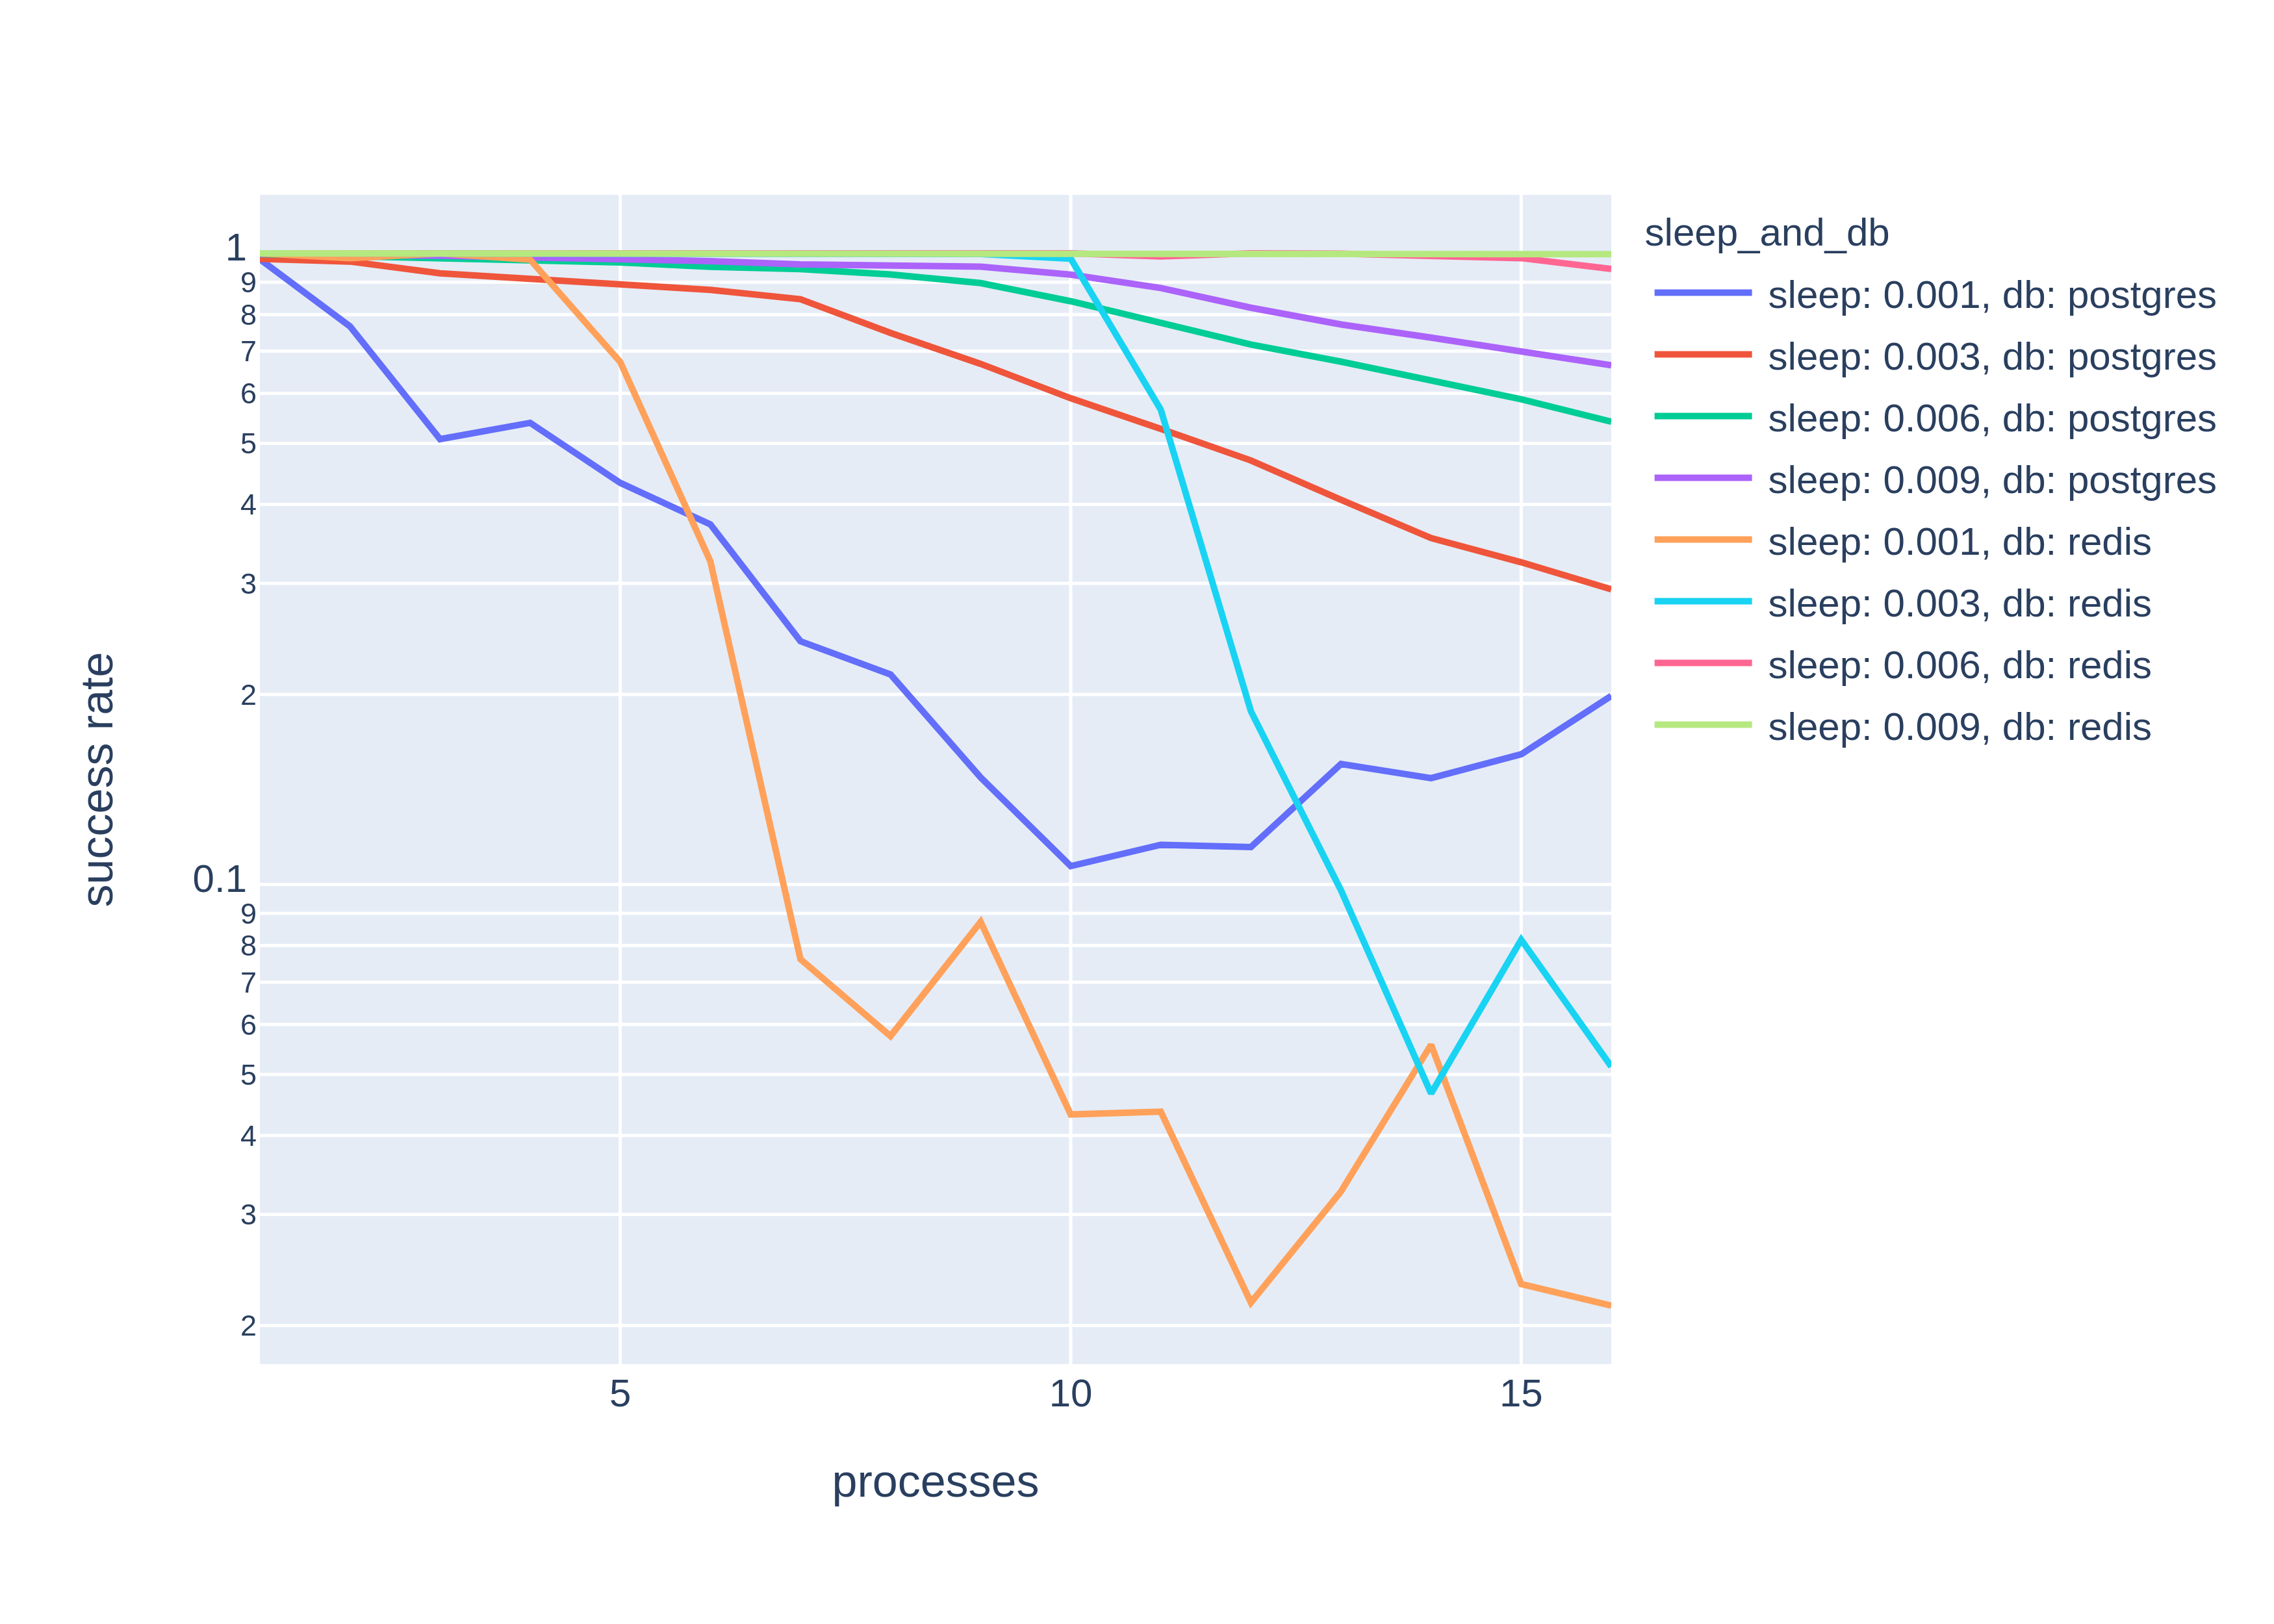
\includegraphics[width=0.9\textwidth]{./graphs/success_rate_all_sleeps.png}
    \caption{Porównanie prawdopodobieństwa wyemitowania reklamy poniżej 20ms}
\end{figure}

Podobnie jak dla czasu wykonania, prawdopodobieństwo wyemitowania reklamy dla postgresa spada wolno i przewidywalnie a dla redisa, obserwujemy gwałtowny skok.

\begin{figure}[H]
    \centering
    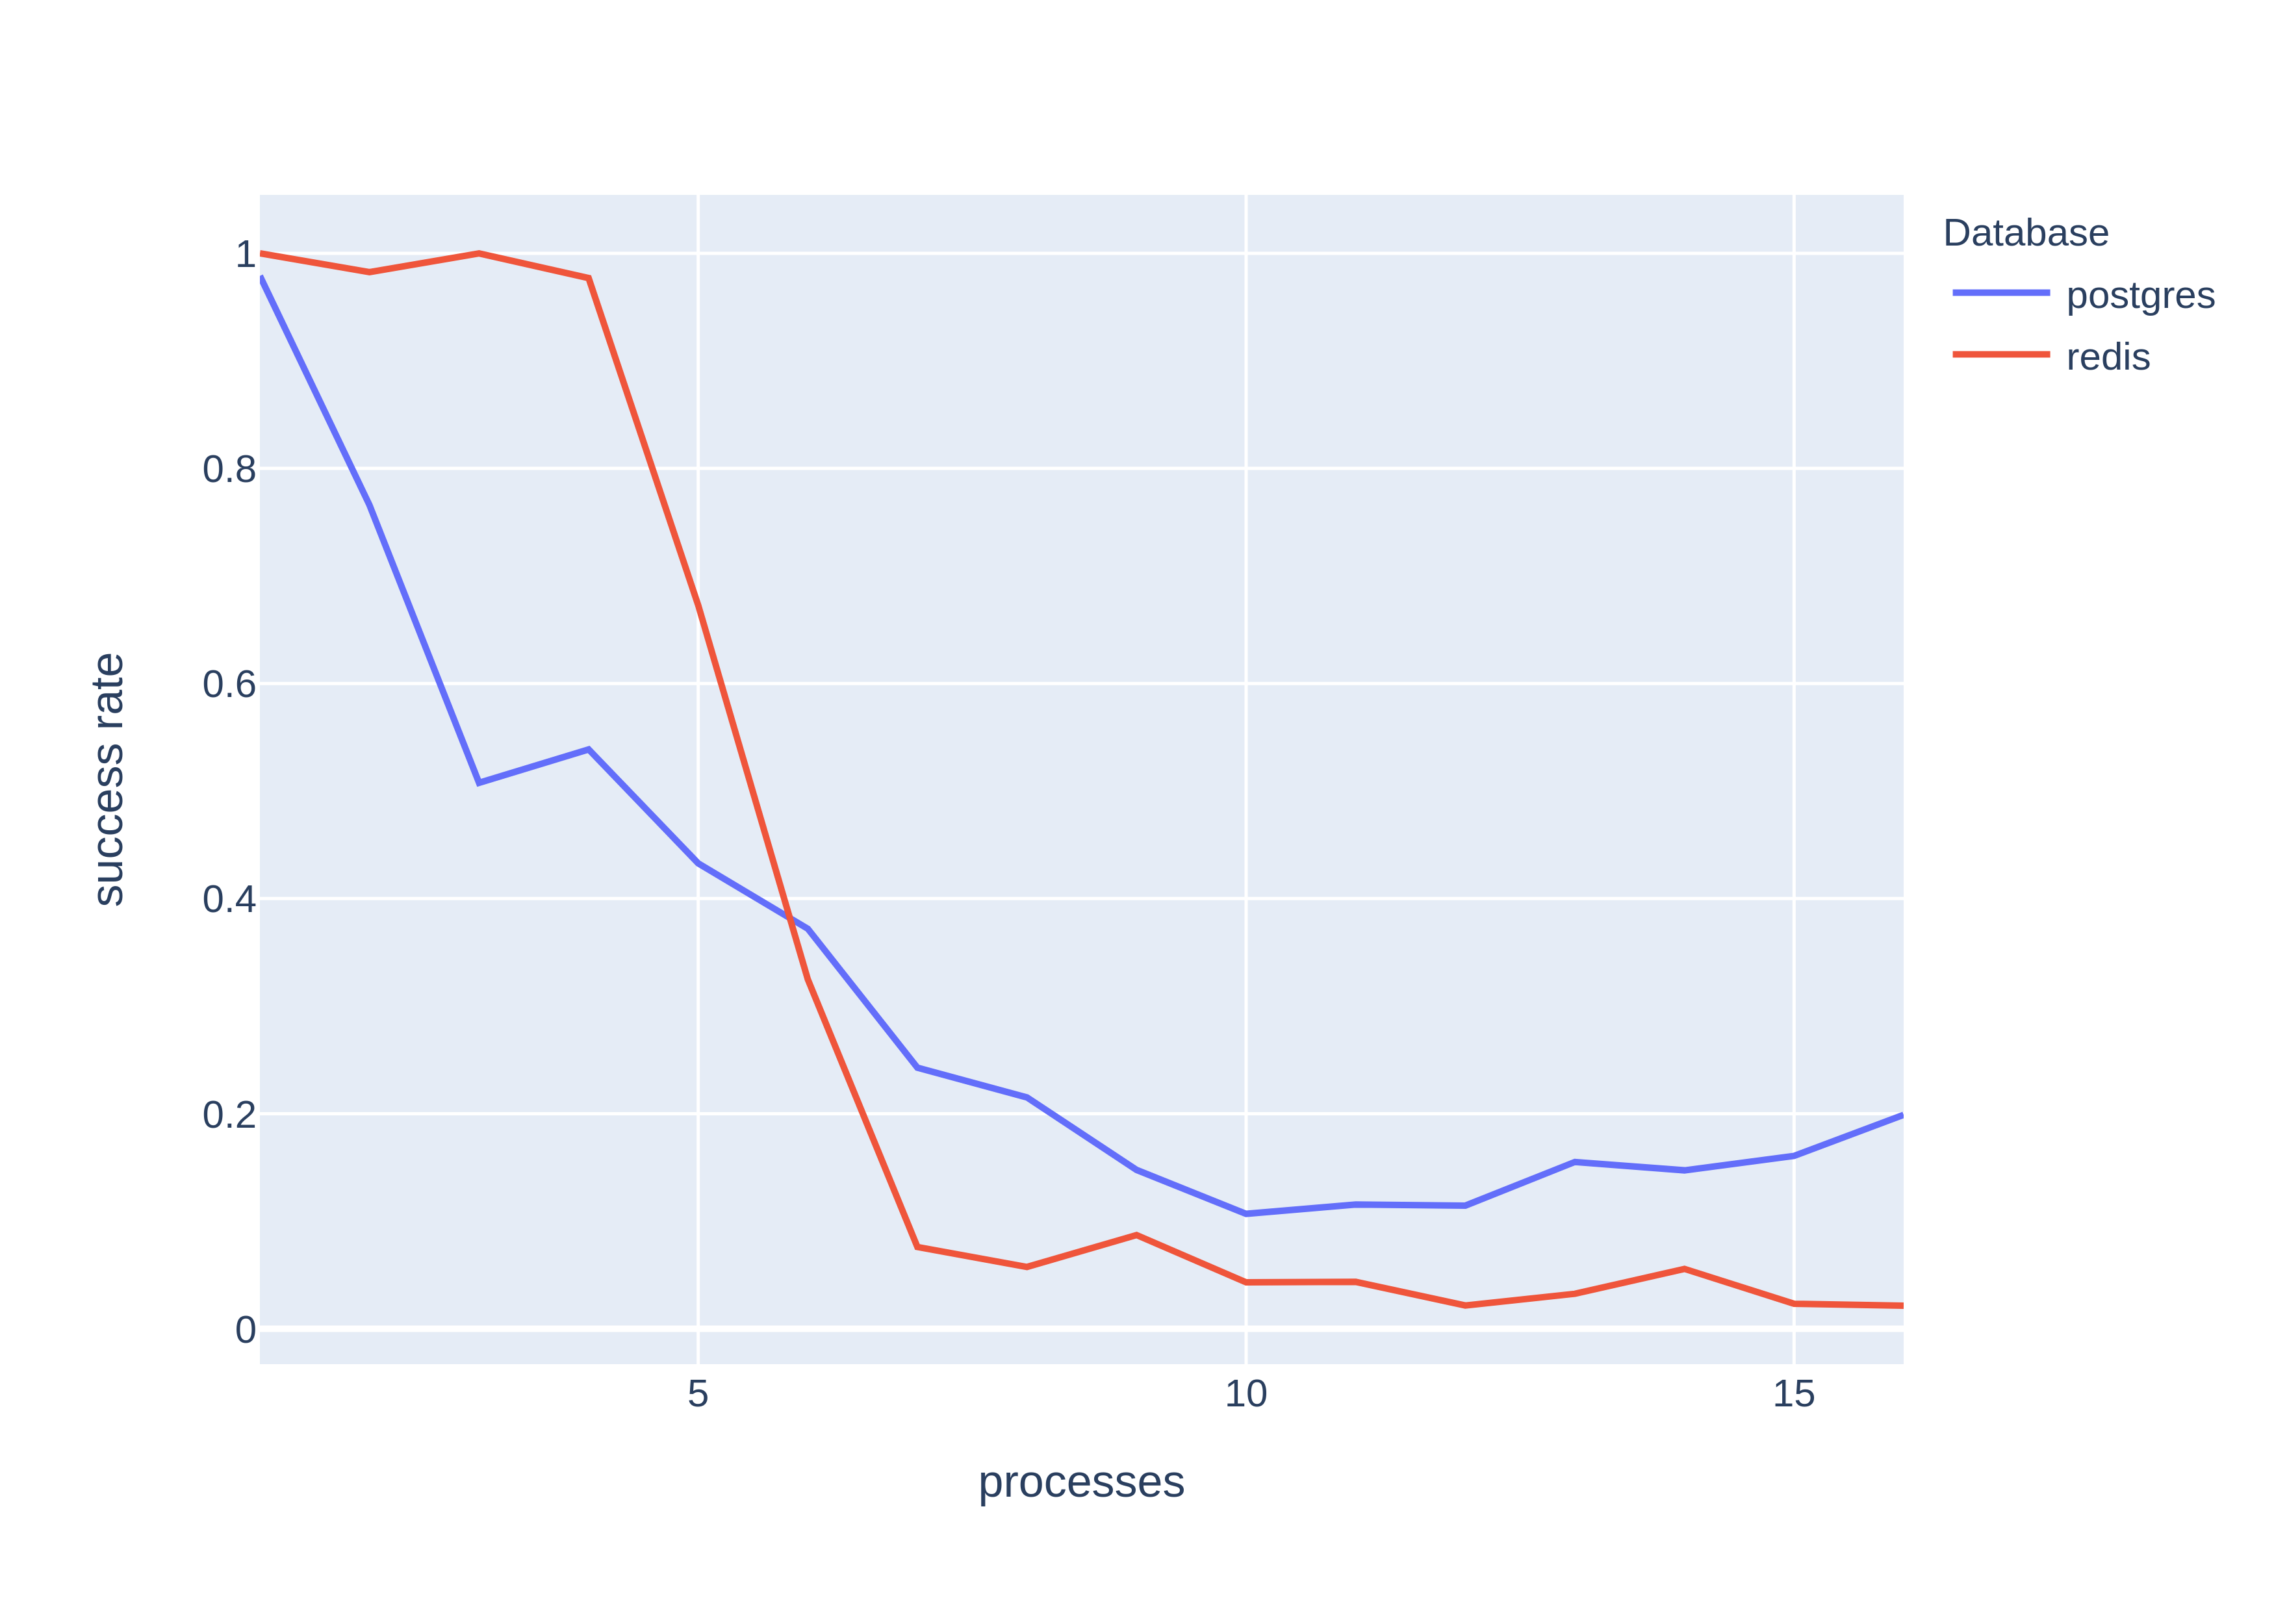
\includegraphics[width=0.9\textwidth]{./graphs/success_rate_postgres_vs_redis_0001.png}
    \caption{Porównanie prawdopodobieństwa wyemitowania reklamy poniżej 20ms w zależności od bazy danych dla t = 0.0001}
\end{figure}

\begin{figure}[H]
    \centering
    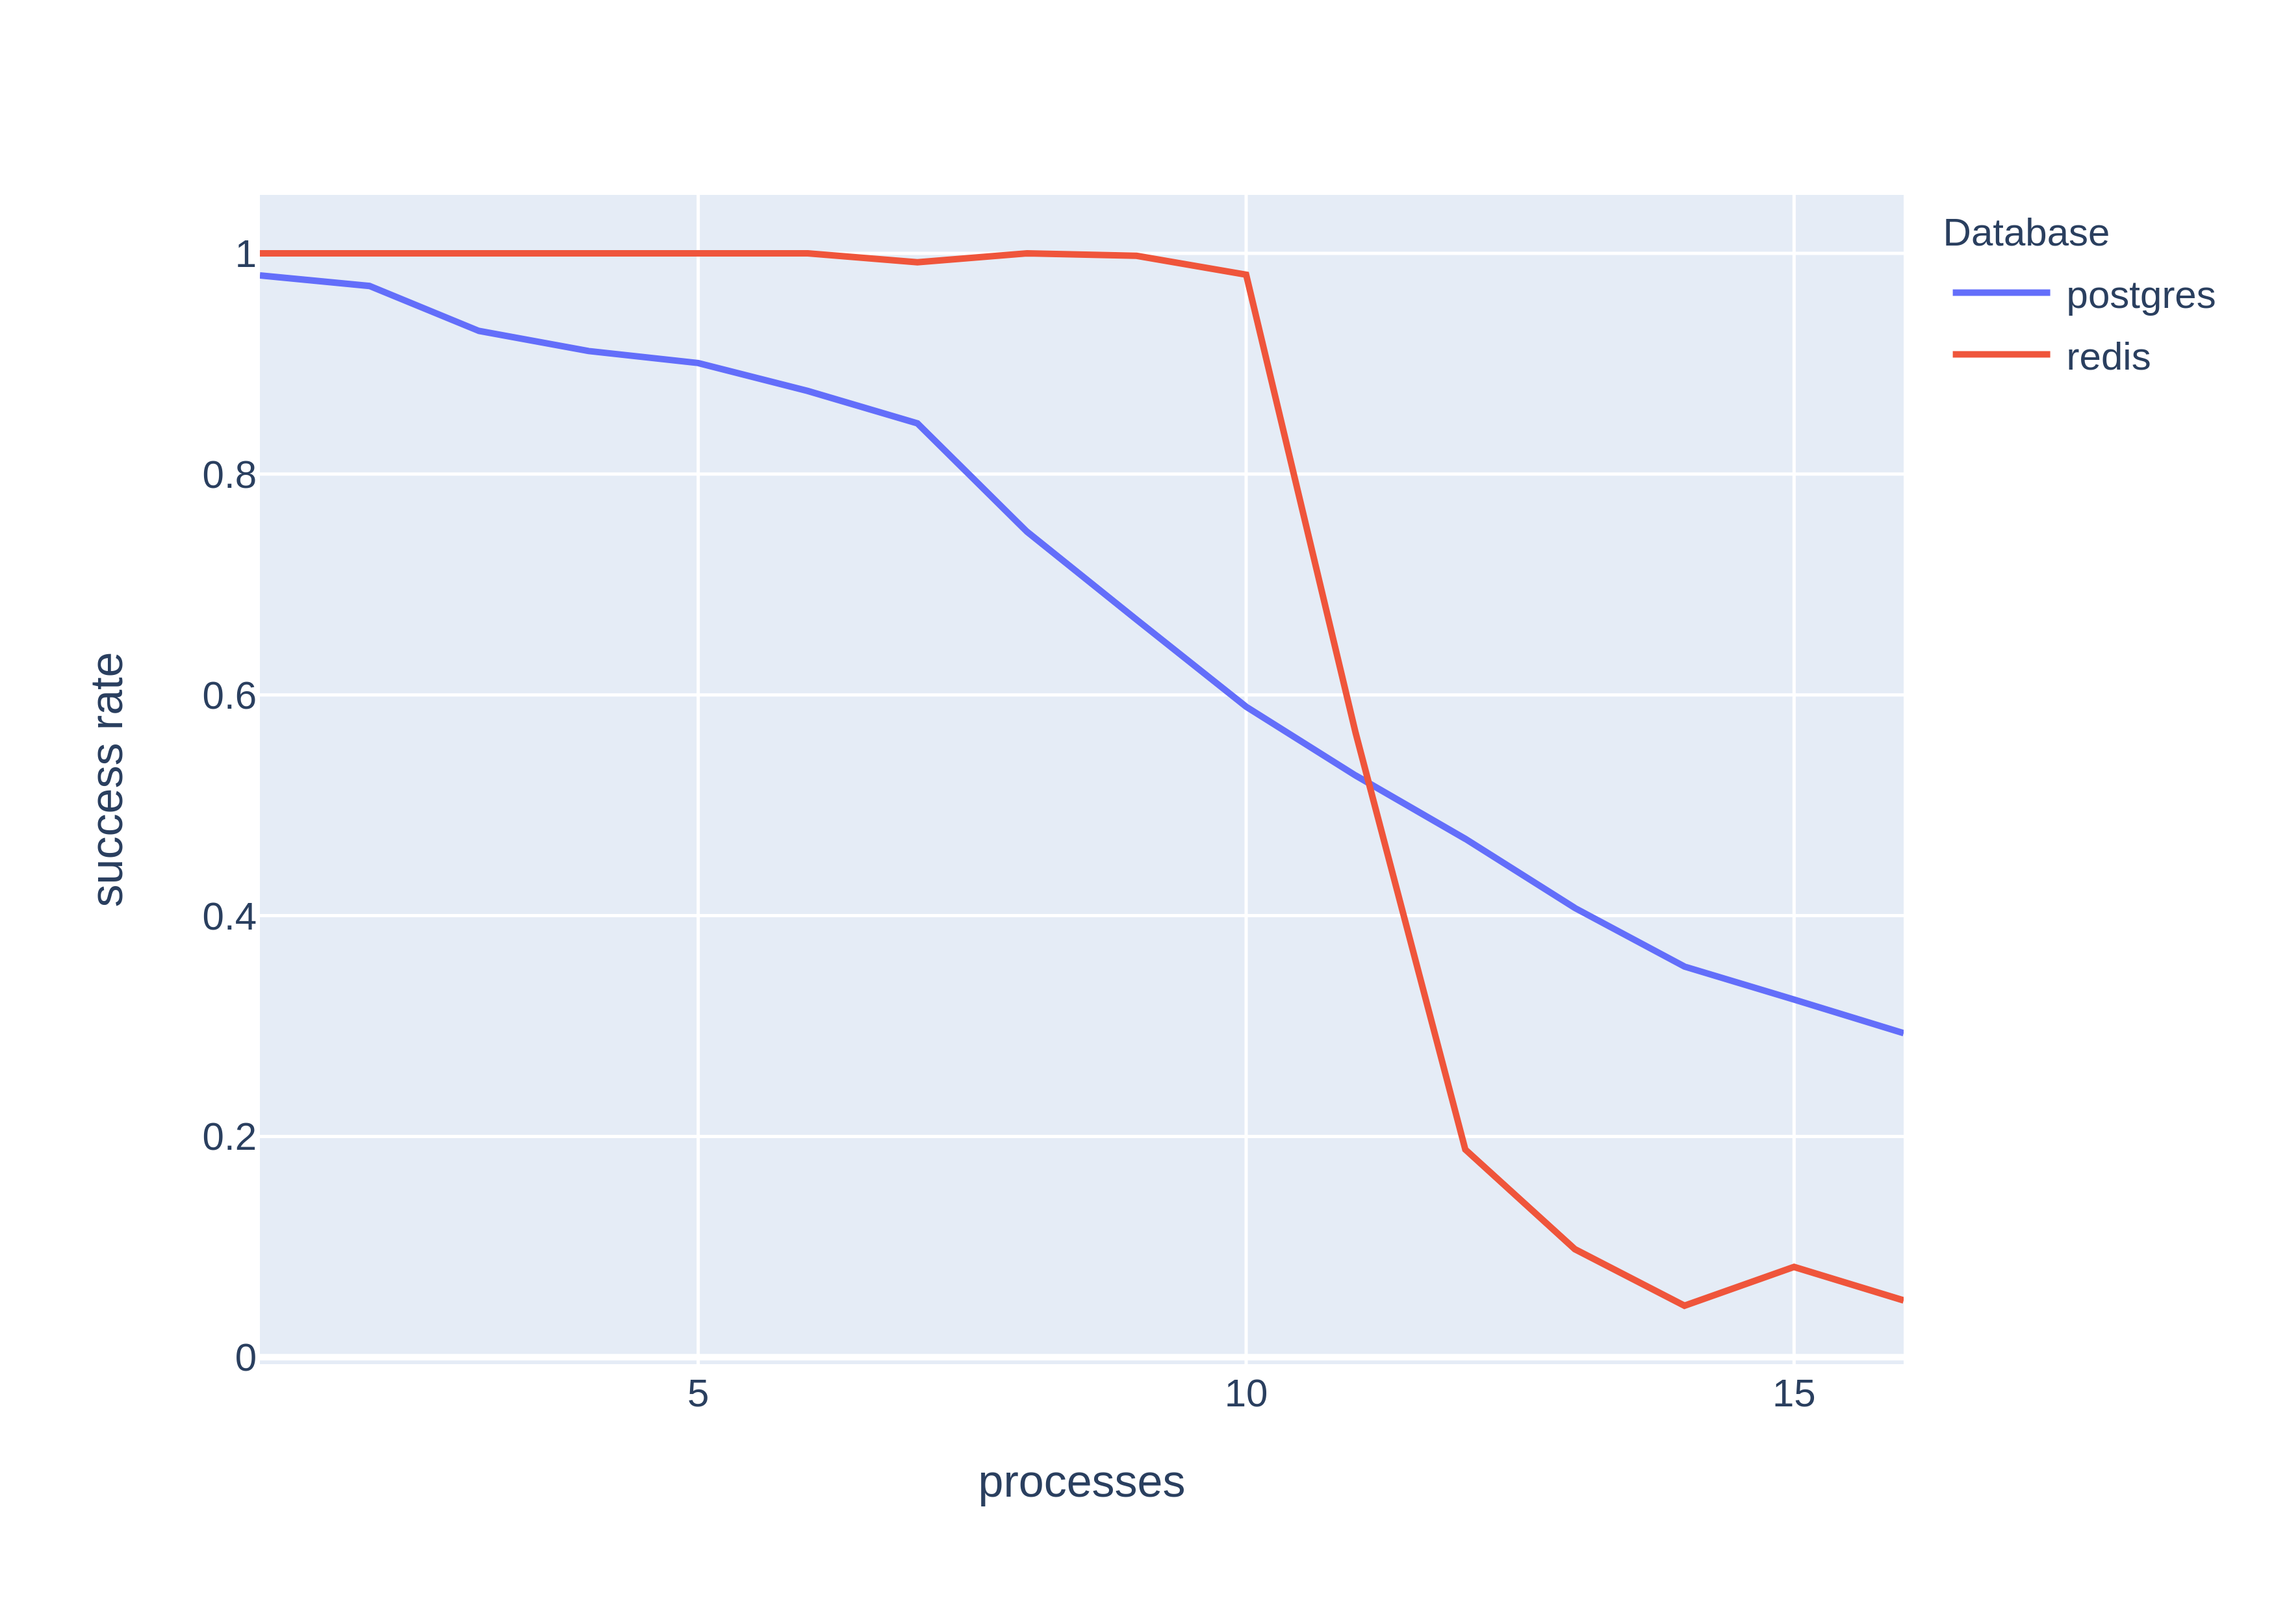
\includegraphics[width=0.9\textwidth]{./graphs/success_rate_postgres_vs_redis_0003.png}
    \caption{Porównanie prawdopodobieństwa wyemitowania reklamy poniżej 20ms w zależności od bazy danych dla t = 0.0003}
\end{figure}

\begin{figure}[H]
    \centering
    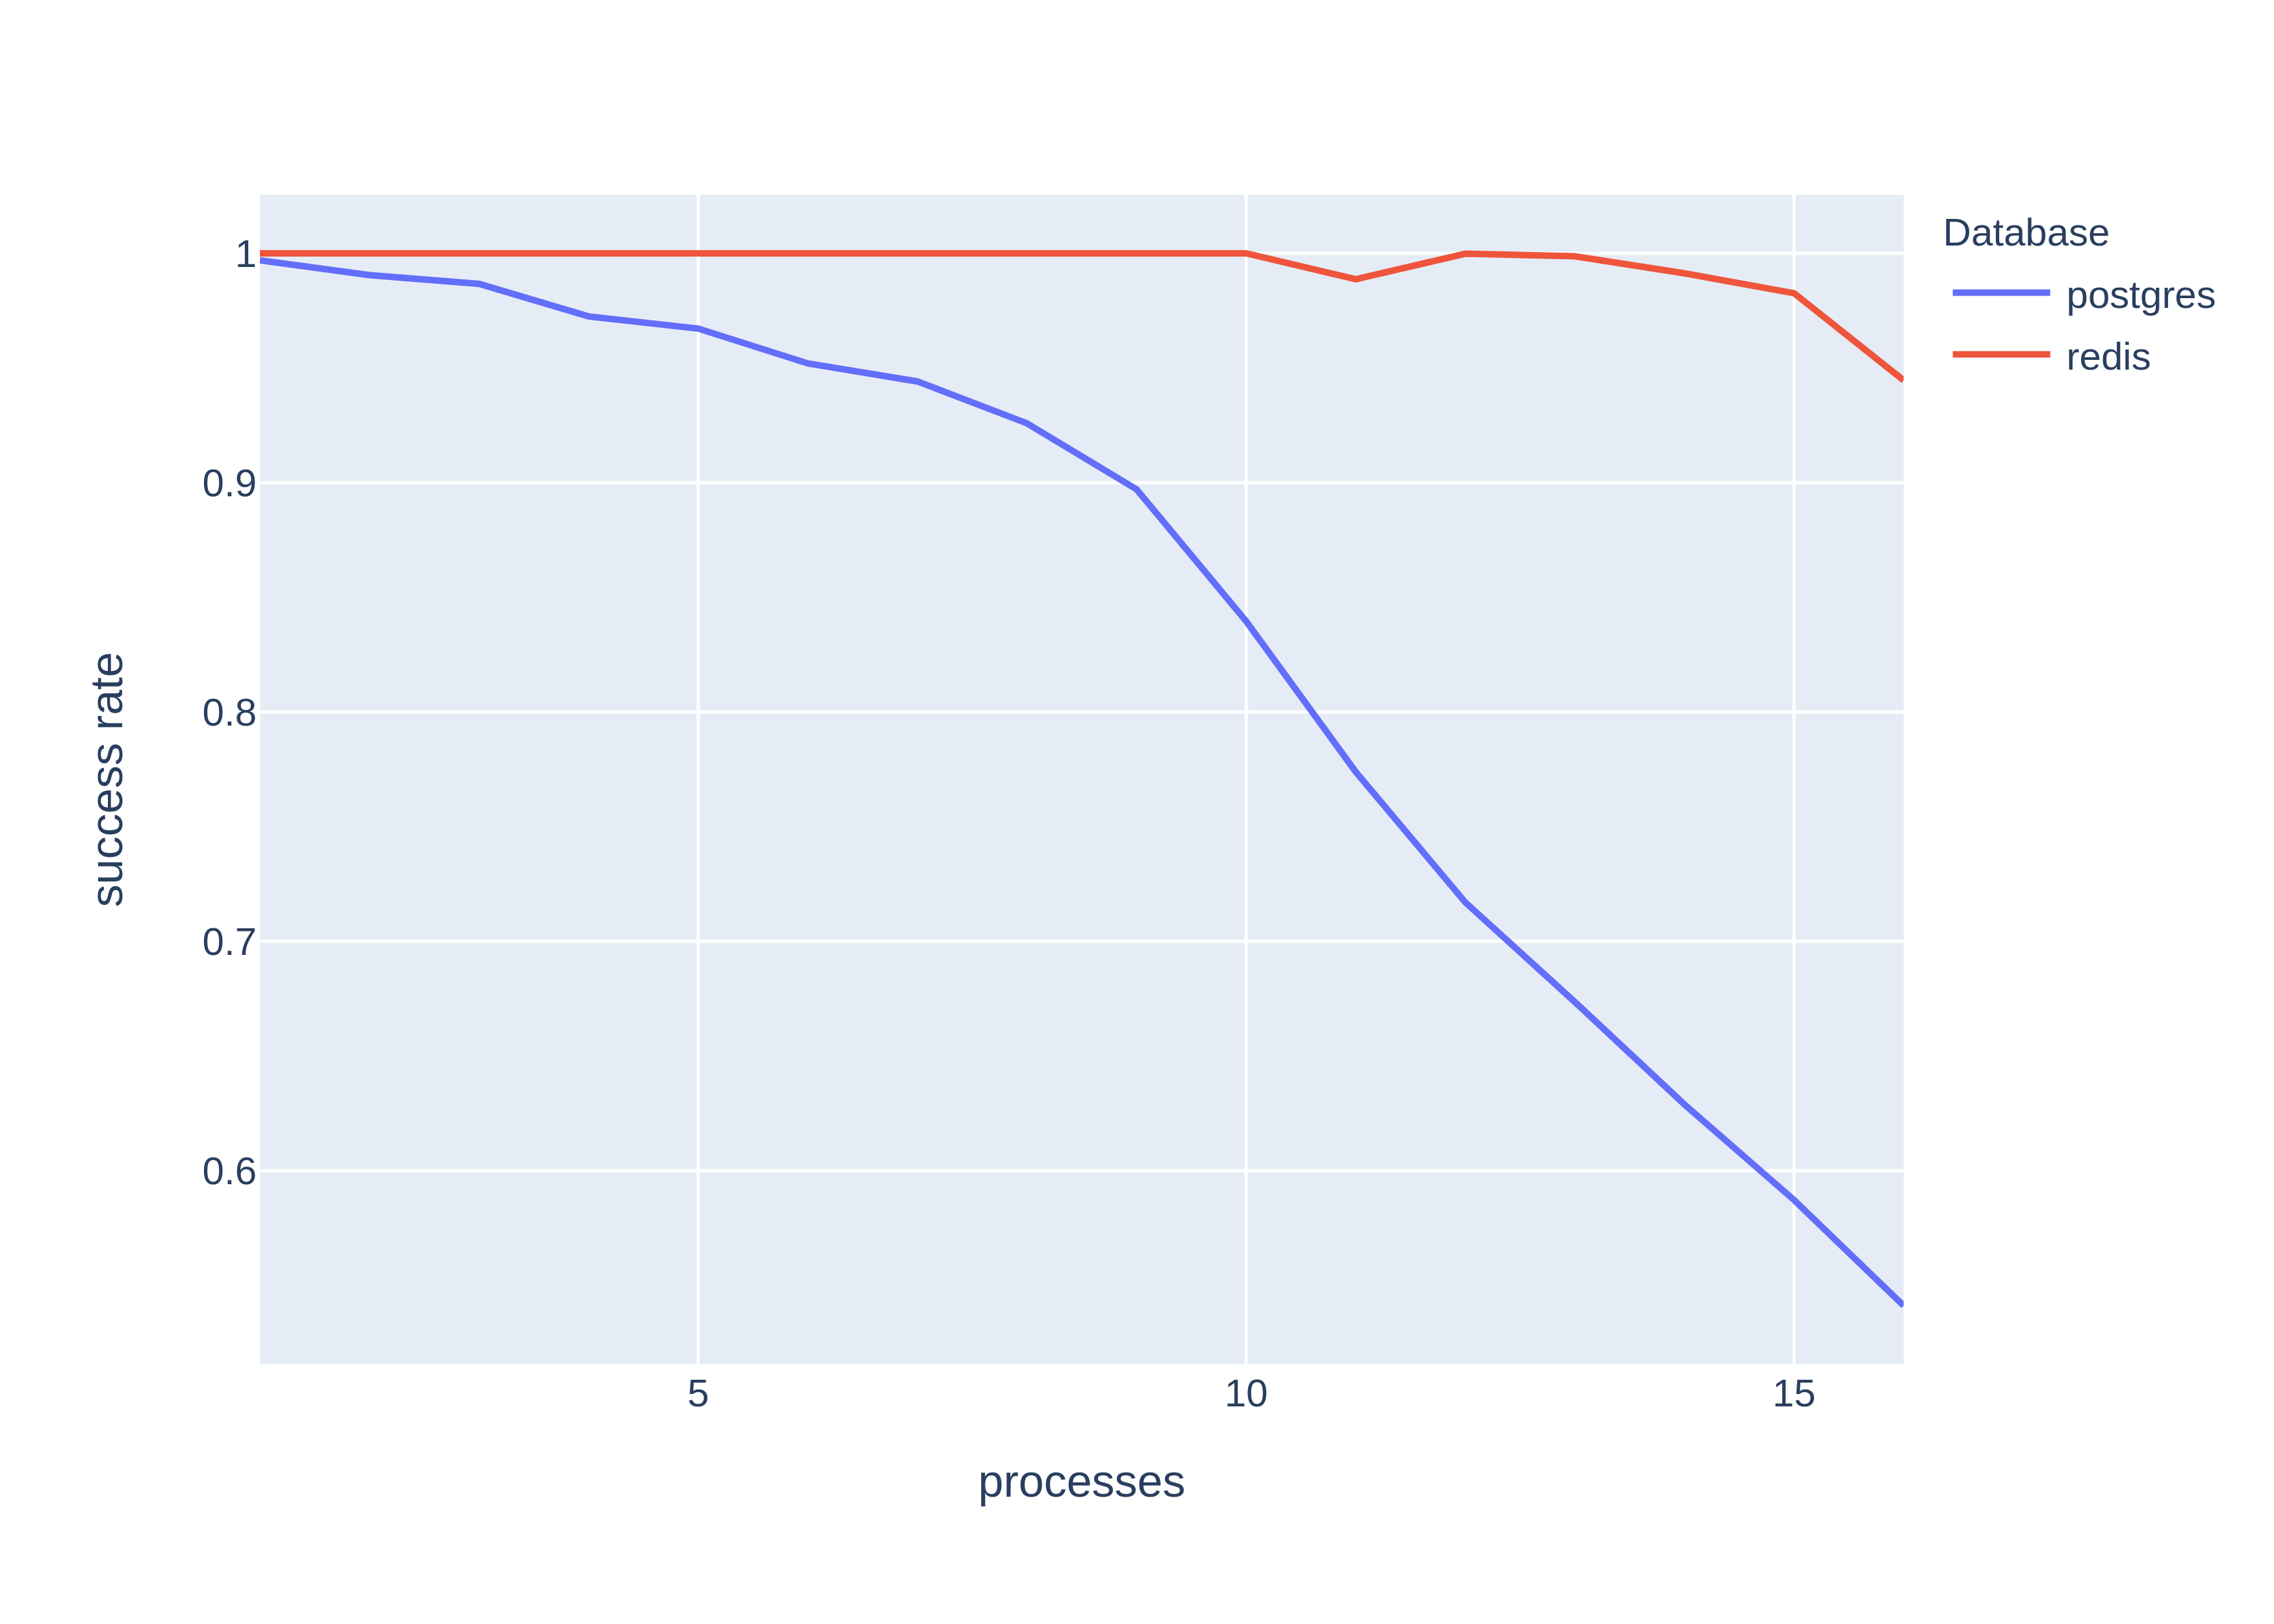
\includegraphics[width=0.9\textwidth]{./graphs/success_rate_postgres_vs_redis_0006.png}
    \caption{Porównanie prawdopodobieństwa wyemitowania reklamy poniżej 20ms w zależności od bazy danych dla t = 0.0006}
\end{figure}

\begin{figure}[H]
    \centering
    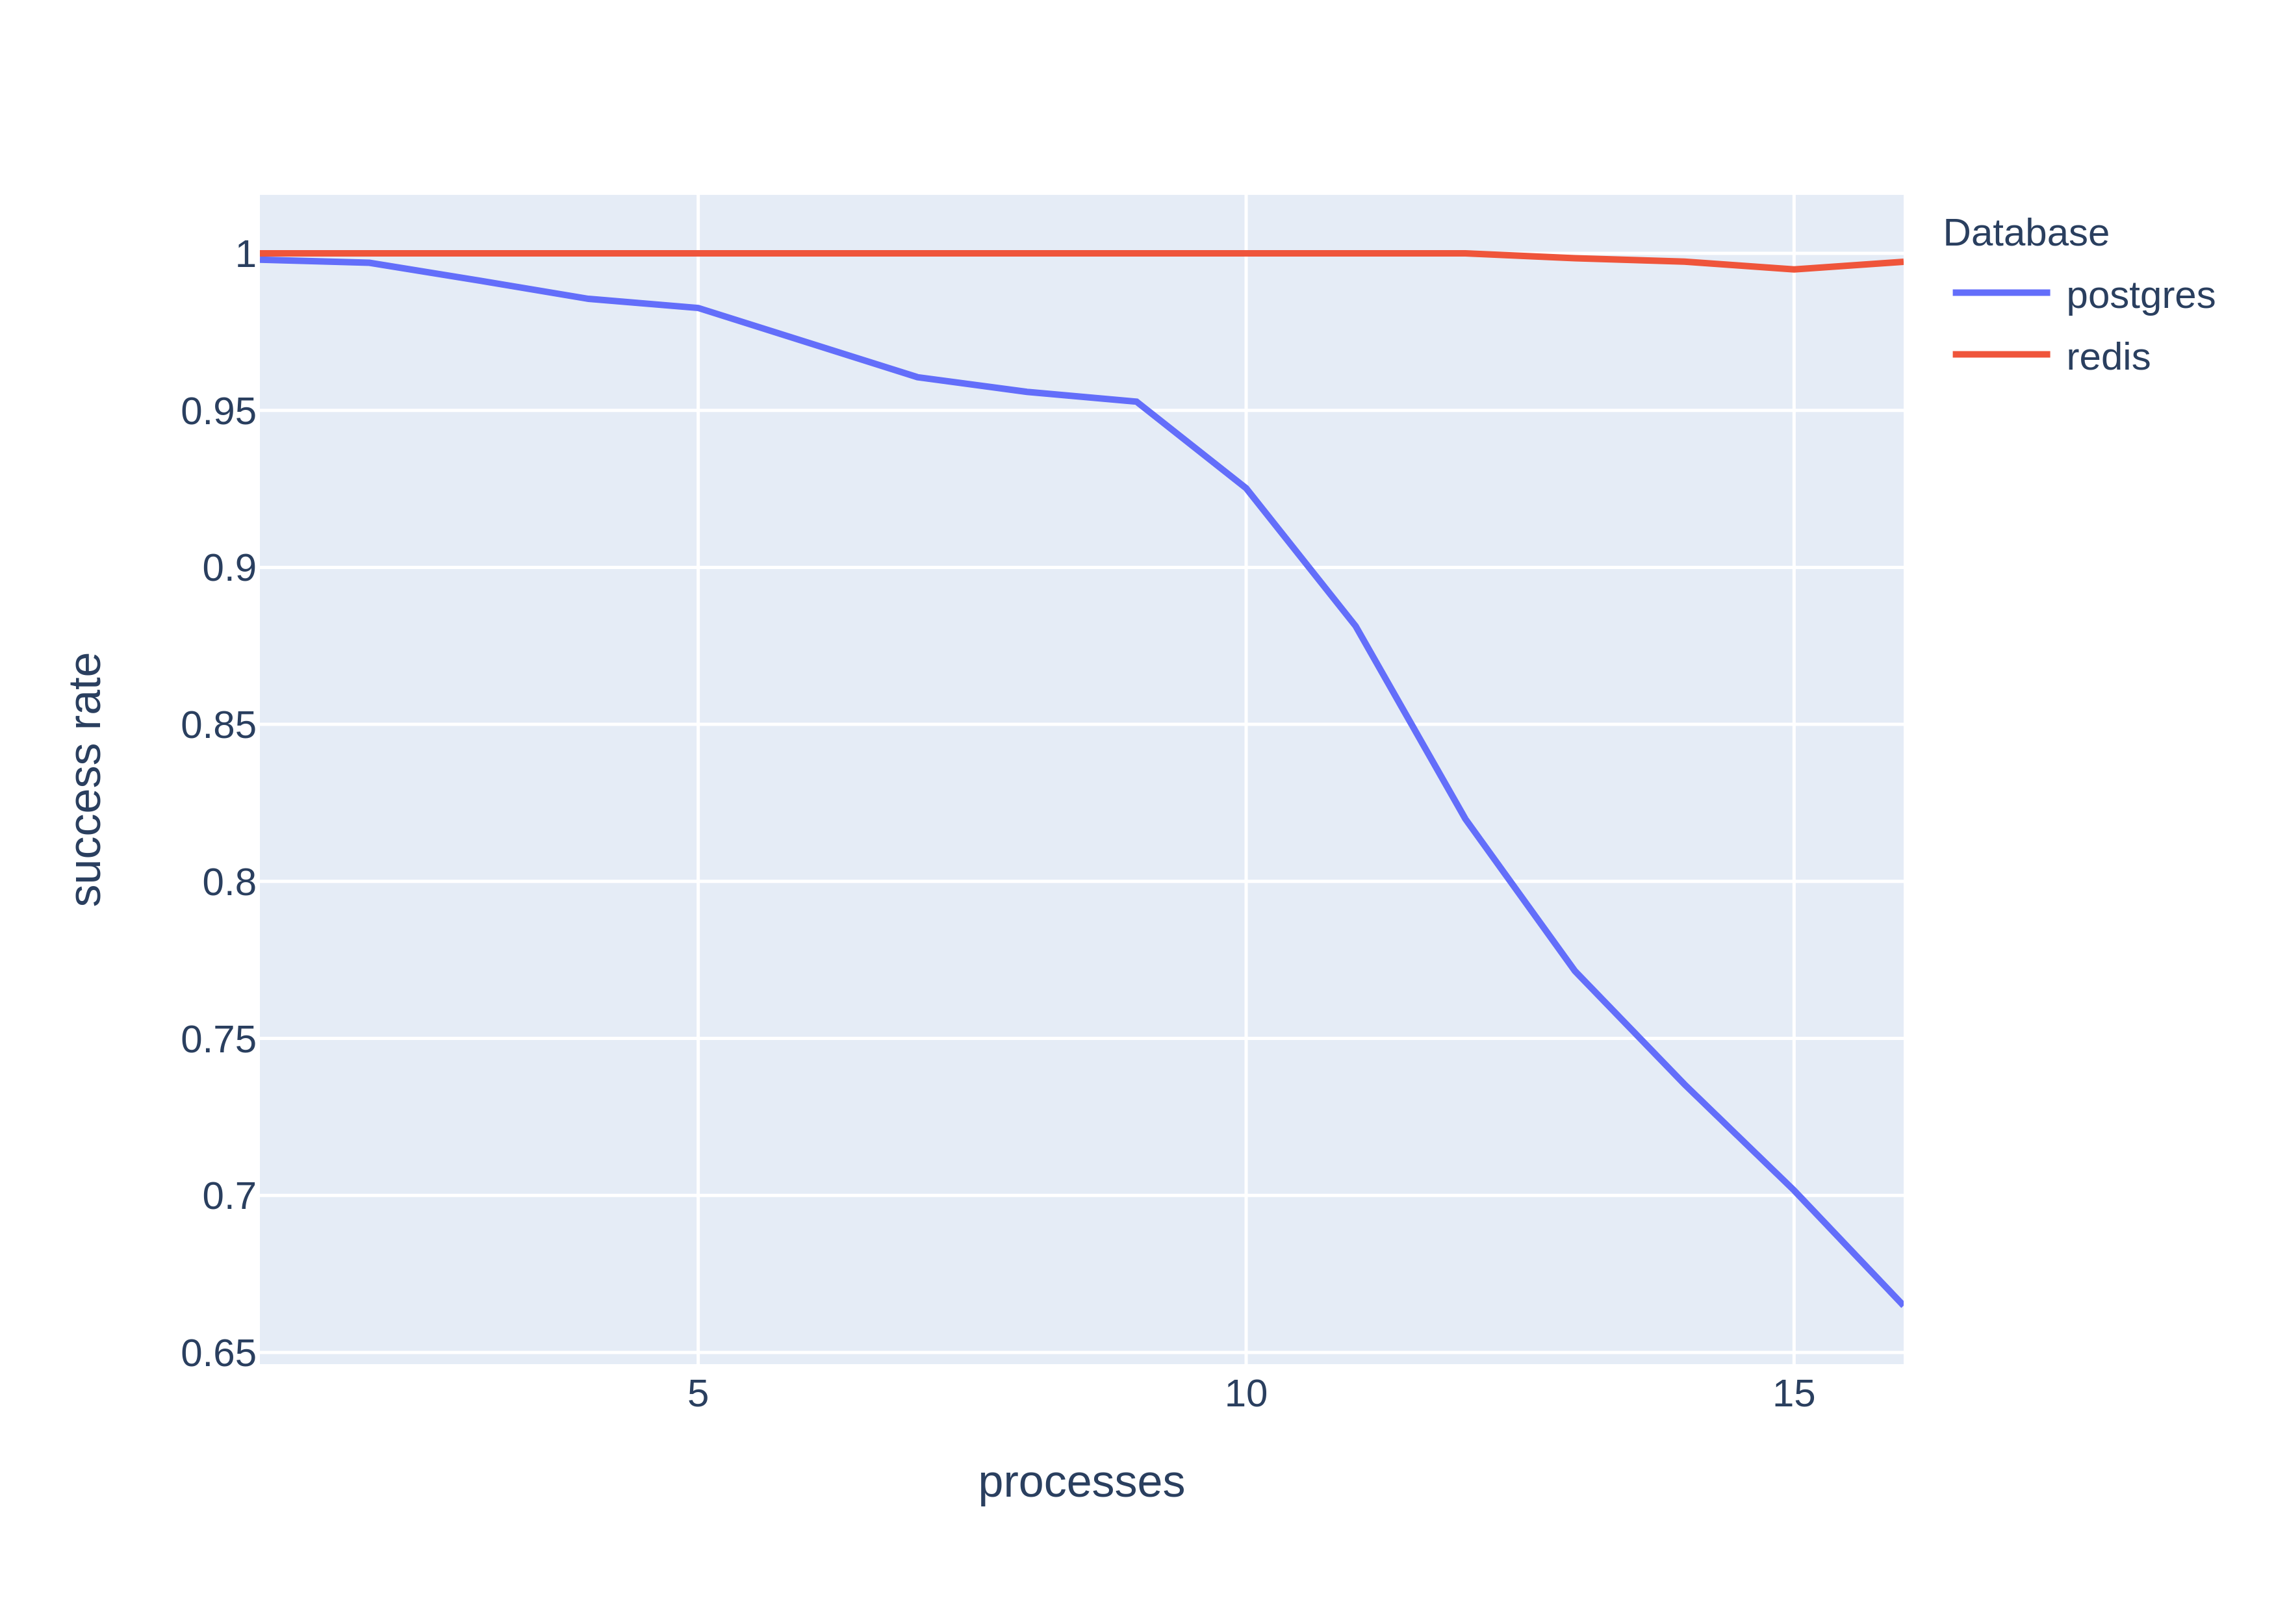
\includegraphics[width=0.9\textwidth]{./graphs/success_rate_postgres_vs_redis_0009.png}
    \caption{Porównanie prawdopodobieństwa wyemitowania reklamy poniżej 20ms w zależności od bazy danych dla t = 0.0009}
\end{figure}

Jeżeli obciążenie bazy ma być bardzo wysokie, lepszym rozwiązaniem może być użycie postgresa zamiast redisa, jeżeli zależy nam jedynie na obsłudze zapytań poniżej 20ms a sama szybkość odpowiedzi w przy normalnym obciążeniu nie jest sprawą drugorzędna.

\subsection{Szybkość obsługi reklamy w zależności od decyzji procesu trzeciego}

\begin{figure}[H]
    \centering
    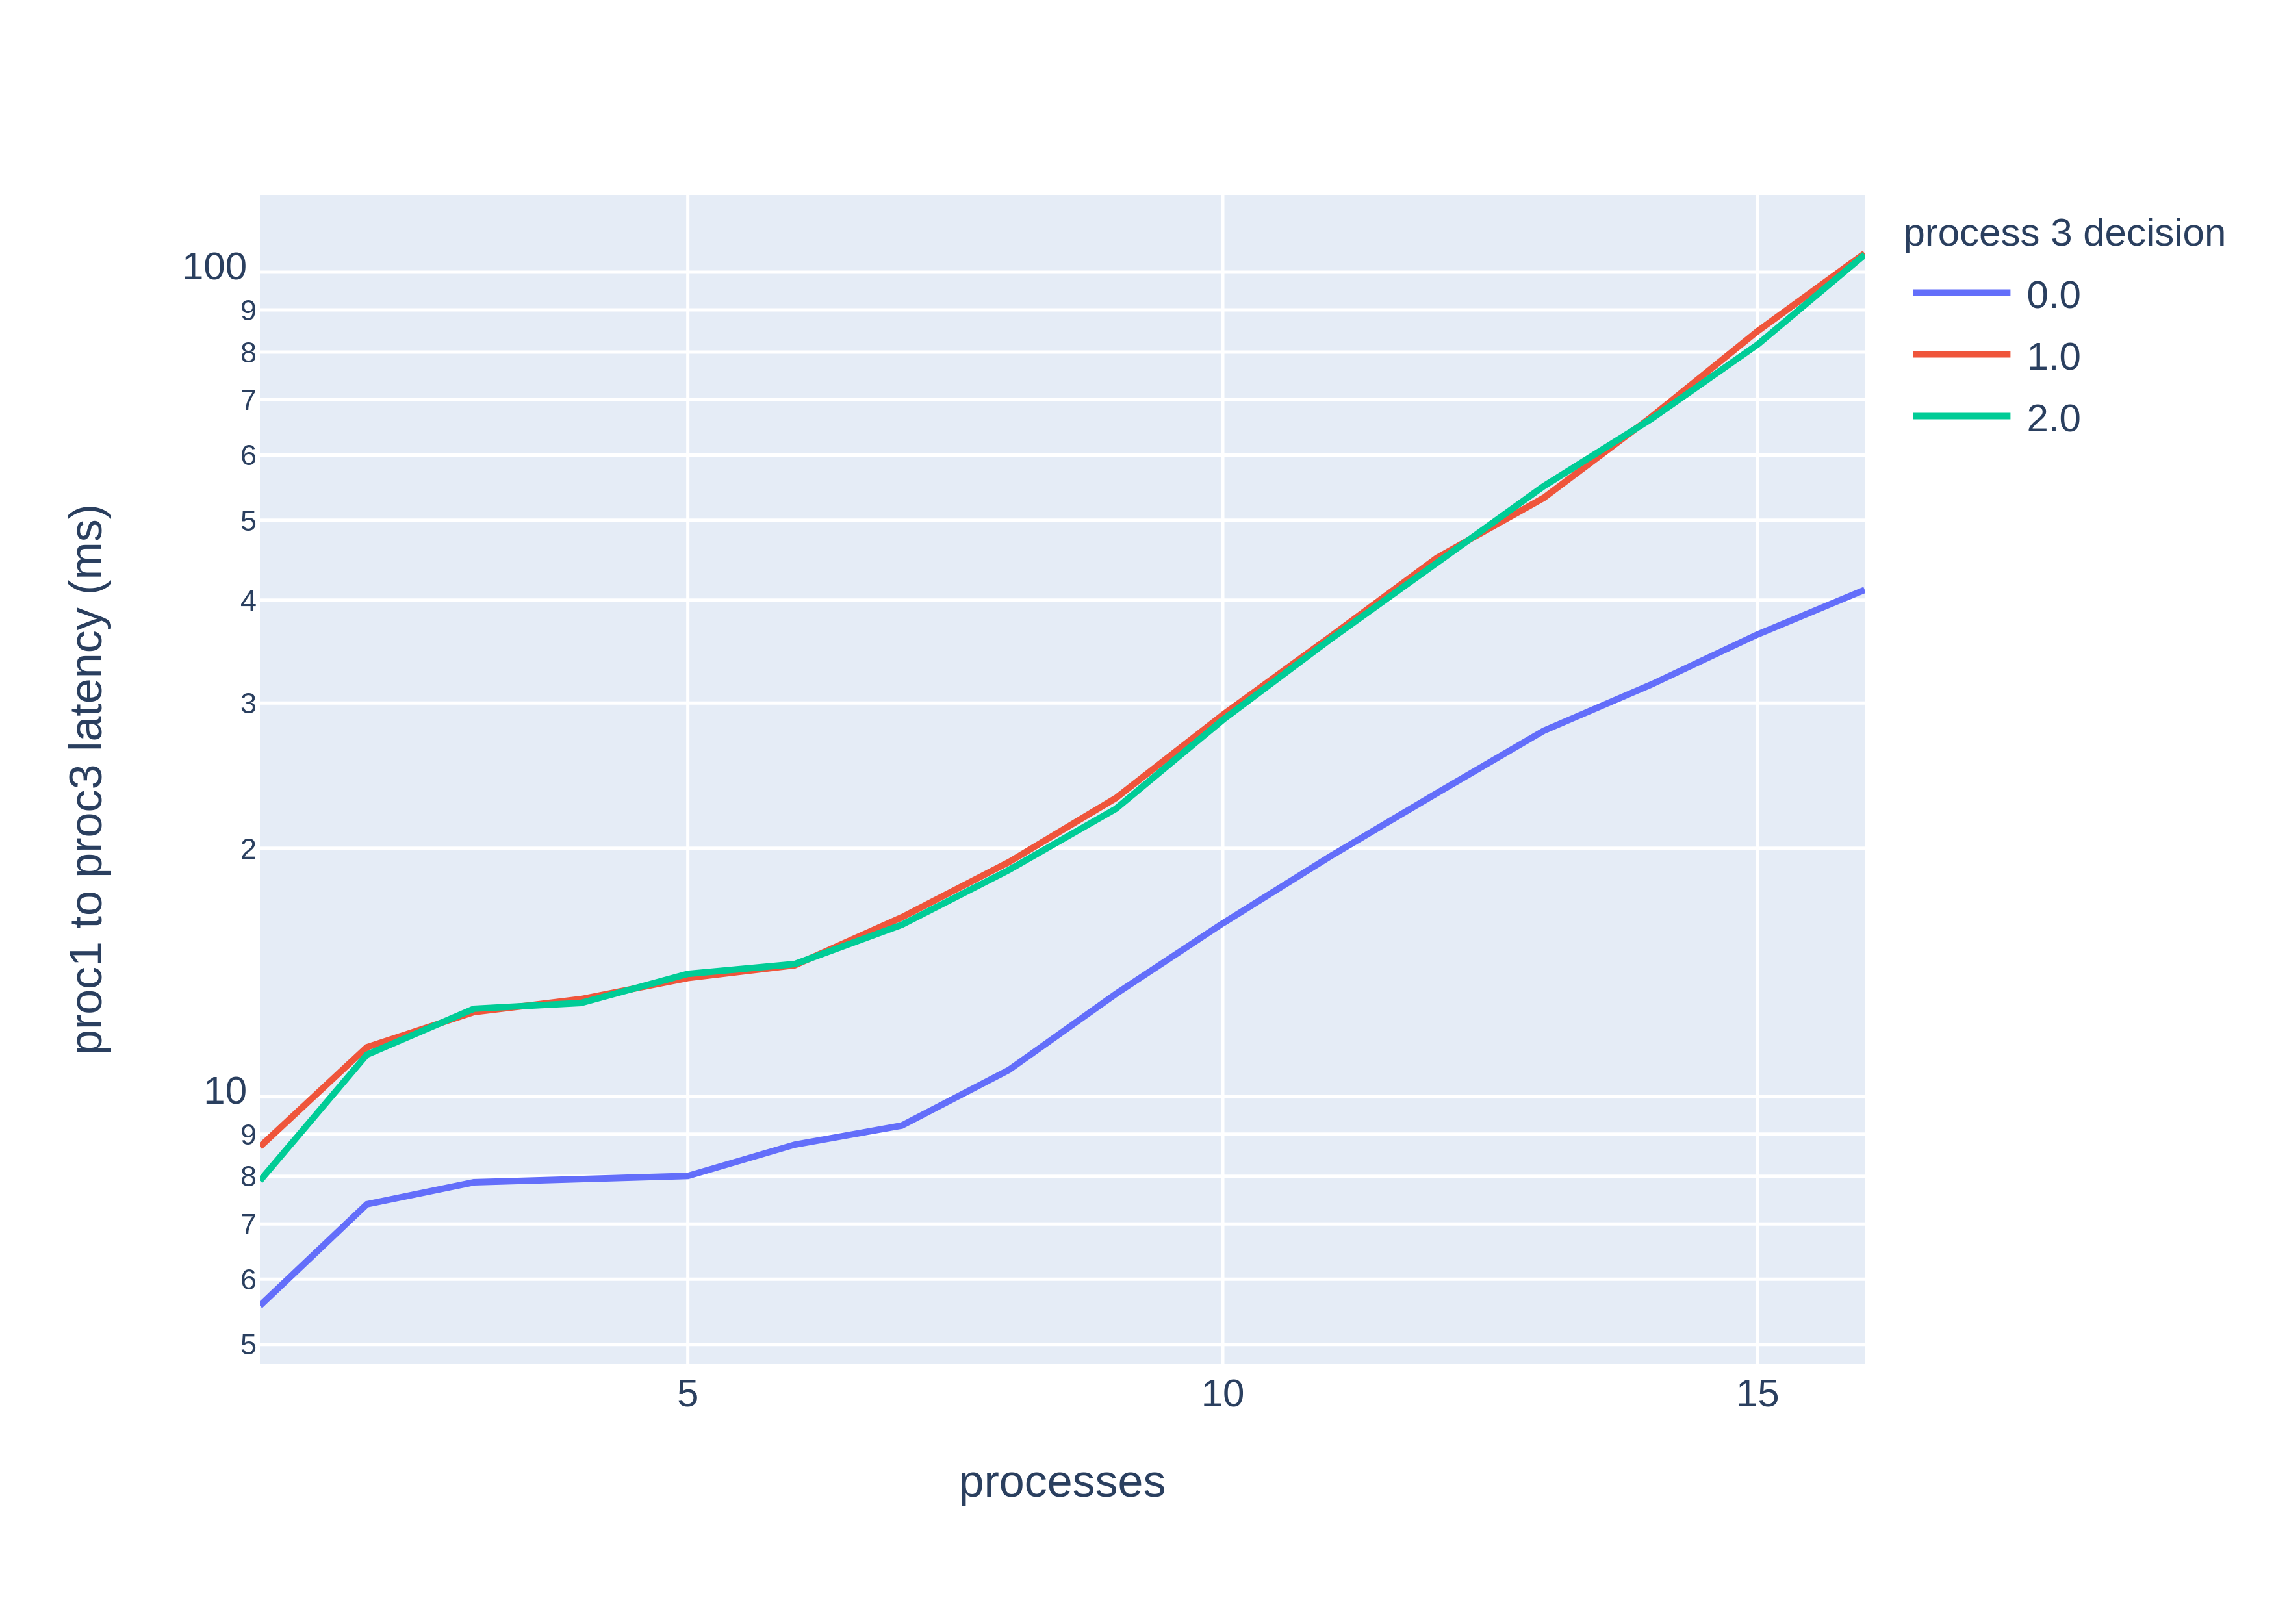
\includegraphics[width=0.9\textwidth]{./graphs/proc_type_postgres.png}
    \caption{Czas obsługi reklamy dla postgresa w zależności od decyzji o wyemitowaniu reklamy - (0 - emituj natychmiast, 1 - emituj po otrzymaniu danych od procesu drugiego, 2 - nie emituj )}
\end{figure}

\begin{figure}[H]
    \centering
    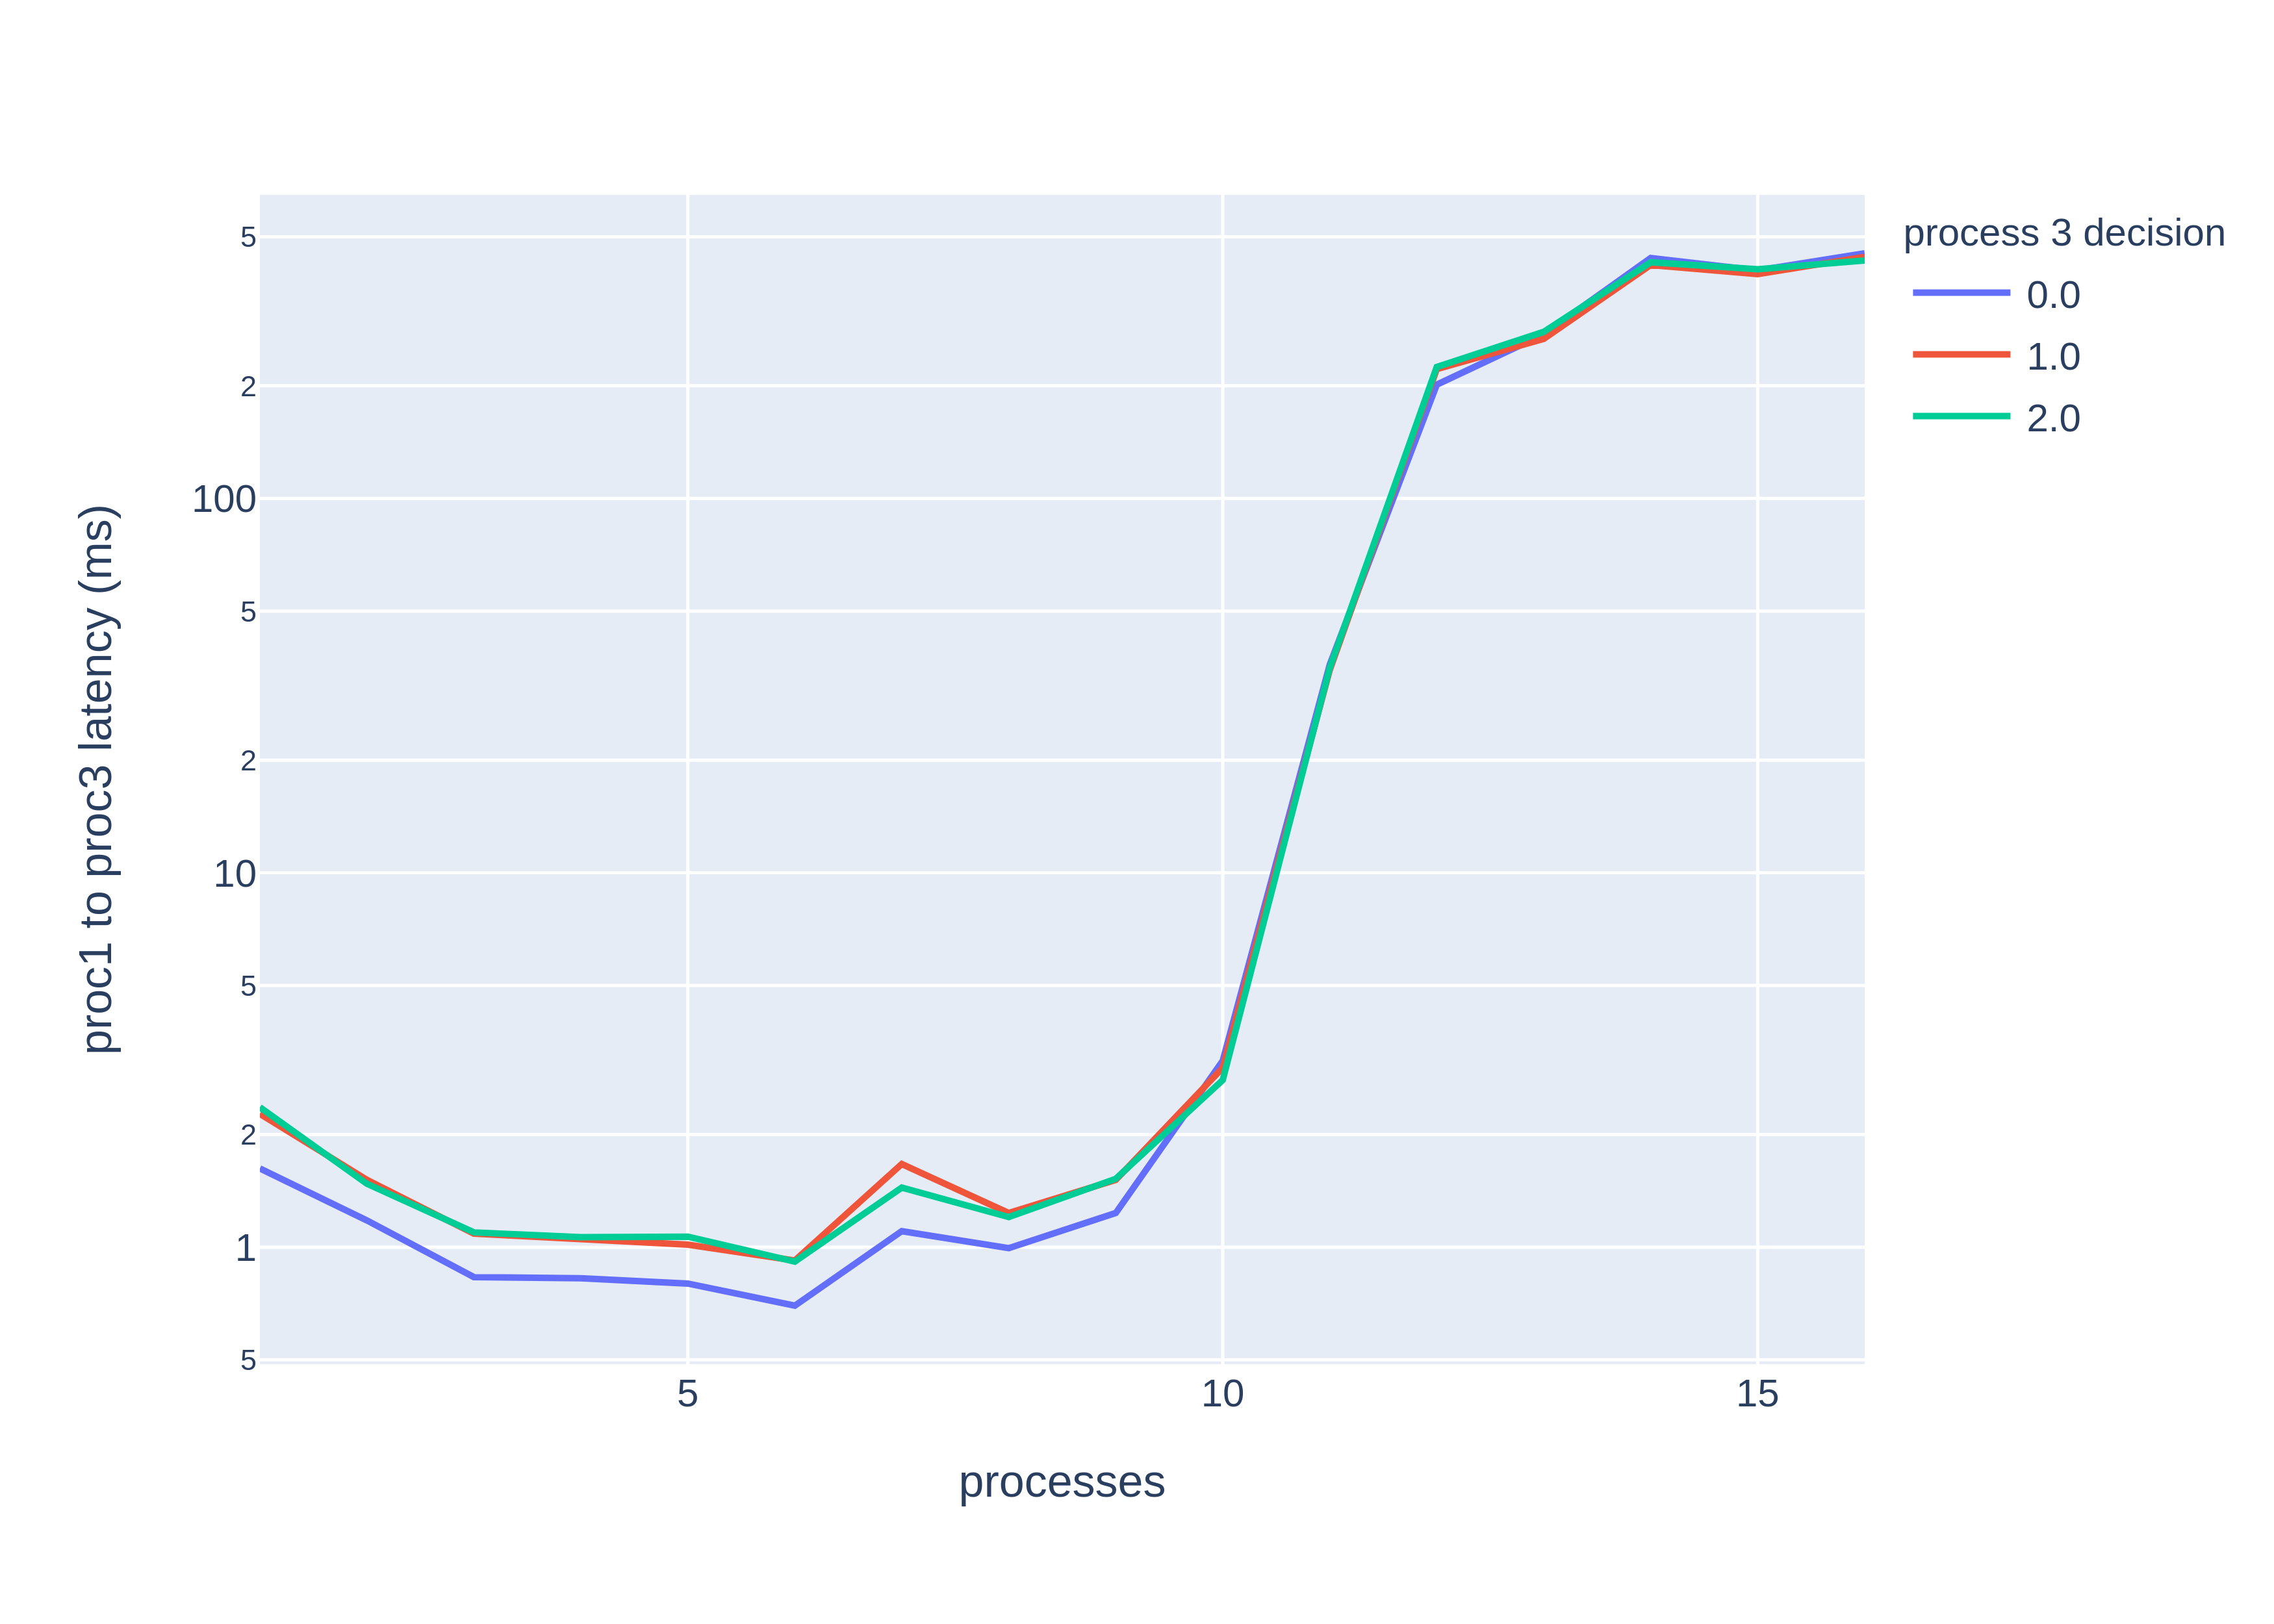
\includegraphics[width=0.9\textwidth]{./graphs/proc_type_redis.png}
    \caption{Czas obsługi reklamy dla redisa w zależności od decyzji o wyemitowaniu reklamy - (0 - emituj natychmiast, 1 - emituj po otrzymaniu danych od procesu drugiego, 2 - nie emituj )}
\end{figure}

Jeżeli proces trzeci potrzebuje danych z procesu drugiego, czas obsługi wydłuża się dwukrotnie w porównaniu z procesem dla którego informacje z procesu pierwszego są wystarczające. Dla postgresa takie zachowanie utrzymuje bez różnicy na liczbę procesów połączonych z bazą. Przy dużym obciążeniu, czas obsługi zapytań przez redisa jest taki bez różnicy jaką decyzje podejmie proces trzeci.

\section{Podsumowanie}
Wbrew oczekiwaniom redis nie jest zawsze bazą szybszą od postgresa. Postgres zachowuje się dużo bardziej przewidywalnie od redisa i może być lepszym wyborem, jeżeli chcemy rozwiązania wolniejszego ale stabilniejszego.



\end{document}
